% !TeX program = xelatex

\documentclass[deliverable]{csreport}

\graphicspath{{./images/}}

\lstloadlanguages{C++,Python}
\usepackage{tikz}
\usetikzlibrary{arrows.meta}

% ---- Per-language syntax-highlight colour schemes ----
\definecolor{cpkw}{RGB}{0,0,200}      % C++ keywords: deep blue
\definecolor{pykw}{RGB}{128,0,200}    % Python keywords: purple
\definecolor{lststr}{RGB}{163,21,21}  % strings (both): dark red
\definecolor{lstcmt}{RGB}{0,128,0}    % comments (both): green

\lstdefinestyle{cppcolors}{%
  keywordstyle     = \color{cpkw}\bfseries,%
  stringstyle      = \color{lststr},%
  commentstyle     = \color{lstcmt}\itshape,%
  showstringspaces = false%
}
\lstdefinestyle{pycolors}{%
  keywordstyle     = \color{pykw}\bfseries,%
  stringstyle      = \color{lststr},%
  commentstyle     = \color{lstcmt}\itshape,%
  showstringspaces = false%
}

% cscommon.sty defines \code via \newverbcommand (verb-style, reads delimiter as next char).
% Redefine it as a regular text-mode command so \code{...} works everywhere, including
% in moving arguments, description labels, and table cells.
\AtBeginDocument{%
  \renewcommand{\code}[1]{\texttt{\textcolor{CSMaroon}{#1}}}%
}
\newcommand{\tcode}[1]{\texttt{\textcolor{CSMaroon}{#1}}}

\begin{document}

% Front matter

\title{Inspection Testbed Implementation}
\subtitle{Brownfield collective awareness in Aerostack2 for task allocation and collision avoidance in photovoltaic inspections }
\author{Guillermo GP-Lenza (UPM)}
\date{2026/04/28}
\reference{CS-D7.4}
\version{0.1}
\dissemination{Public}
\delno{D7.4}

\maketitle

\executivesummary

This document reports on the implementation of the CORESENSE Drone Inspection Testbed (TB2), describing the software contributions made to the Aerostack2 robotics framework that enable a fleet of autonomous drones to perceive their shared environment, allocate inspection targets, and navigate safely in the presence of peers.

The implementation is grounded in the collective awareness architecture defined in D7.3 \\ \cite{CORESENSE-D73}.
According to that document, \emph{awareness for a multi-robot system~$S$ is the synchronous understanding of the situation by~$S$}.
Achieving this requires agents to maintain self-models and collective models, communicate modelets between each other, and integrate information into shared knowledge structures.
The CORESENSE definition of cognitive modules---\emph{subsystems that realise the modelet-engine concept, using representations (models) to derive relevant information by suitable algorithms (engines)}---maps naturally onto Aerostack2 \emph{behaviors}, the plugin-based action-server components that encapsulate robot skills.

The document is structured around the infrastructure-first narrative proposed in D7.3: first the communication backbone, then the knowledge layer, and finally the behaviors that use both.

\begin{itemize}
  \item \textbf{Collective Awareness middleware (\code{as2\_ca})} --- implements the Collective Awareness Module of the D7.3: a gateway node that handles peer discovery and modelet routing, and a client component that gives behaviors a typed API for sending and receiving modelets.
  \item \textbf{Knowledge Base Interface (\code{as2\_core} and \code{as2\_python\_api})} --- connects Aerostack2 behaviors and mission scripts to the CORESENSE \code{knowledge\_core}, enabling fact assertion, querying, and reactive event handling.
  \item \textbf{Auction Behavior (\code{as2\_behaviors})} --- implements the \emph{auctions} collective model: task allocation through bid exchange over the CA gateway, cost computation from self-model data, and result grounding in the knowledge base.
  \item \textbf{Collision Avoidance Behavior (\code{as2\_behaviors})} --- implements the \emph{consensus} collective model: distributed path-lock arbitration through lock-request exchange over the CA gateway, with path prepended from self-model data.
\end{itemize}

Together, these components satisfy the functional requirements for collaborative planning, failure resilience, trajectory collective-awareness, and safety distance maintenance stated in D7.2 \cite{CORESENSE-D72}, and enable the inspection scenarios defined in D7.1 \cite{CORESENSE-D71}.

We acknowledge the financial support through the contract \#101070254, \emph{CoreSense: A Hybrid Cognitive Architecture for Deep Understanding} granted by the European Commission inside the Horizon Europe programme.

\documentversions
\versionitem{0.1}{Initial draft}{G.~GP-Lenza (UPM)}{2026/04/28}

\tableofcontents

%%%%%%%%%%%%%%%%%%%%%%%%%%%%%%%%%%%%%%%%%%%%%%%%%%%%%%%%%%%%%%%%%%%%%%%%%%%%%

\chapter{Introduction}

\section{Context and motivation}

The CORESENSE project aims to endow autonomous robotic systems with a hybrid cognitive architecture that combines reactive and deliberative reasoning grounded in explicit models. Work Package~7 contributes the Drone Inspection Testbed (TB2): a multi-drone system that autonomously surveys a photovoltaic (PV) power plant, allocates inspection targets among itself, and coordinates its motion.

Deliverable D7.1~\cite{CORESENSE-D71} established the operational concept and stakeholder requirements for TB2, identifying four families of use cases: robot failure and swarm replanning (UC1), emergency landing with dynamic path negotiation (UC2), discrepancy detection in collective sensing (UC3), and assurance of valid inspection images (UC4). Deliverable D7.2~\cite{CORESENSE-D72} translated these into system requirements and proposed an initial Aerostack2-based architecture, identifying the three extensions that CoreSense technologies had to provide:
\begin{enumerate}
  \item \textbf{Inter-agent communication}: drones must exchange structured modelets (bids, lock requests, grants) without a centralised broker.
  \item \textbf{Knowledge grounding}: task assignments and mission events must be recorded in and retrieved from the a knowledge base.
  \item \textbf{Safe multi-robot navigation}: simultaneous access to overlapping flight corridors must be arbitrated before motion begins.
\end{enumerate}

Deliverable D7.3~\cite{CORESENSE-D73} elaborated the Collective Awareness Architecture that addresses these needs, defining the Collective Awareness Module and its three subsystems: \emph{Agent Representation} (the agent's self-model), \emph{Organisation Handling} (collective models and role assignment), and \emph{Communication Interface} (intelligible modelet exchange).

This document, D7.4, reports on the concrete implementation of those three subsystems in Aerostack2.

\section{Aerostack2 and the cognitive module correspondence}

Aerostack2~\cite{AS2-2023} is an open-source, modular framework for autonomous aerial systems built on ROS~2. Its component model separates concerns into \emph{mission control} \emph{behaviors} (action servers), \emph{basic robotic functions}, and \emph{platforms}. Behaviors are pieces of robot intelligence: each encapsulates a robot skill as a ROS~2 action server backed by a loadable plugin.

The CORESENSE architecture defines cognitive modules as \emph{subsystems that realise the modelet-engine concept}: they maintain \emph{models} of relevant phenomena and apply \emph{engines} (inference algorithms) to those models to derive outputs. The inputs and outputs communicated between modules are called \emph{modelets}. This maps directly onto Aerostack2 behaviors: the plugin is the engine, the behavior's internal state is the model, and the typed messages it exchanges are the modelets. Chapter~\ref{ch:cognitive} makes this correspondence precise.

\section{Document structure}

Chapter~\ref{ch:cognitive} establishes the correspondence between Aerostack2 behaviors and CORESENSE cognitive modules. Chapter~\ref{ch:ca} presents the Collective Awareness middleware---the CA Gateway and CA Client---as the implementation of the D7.3 Communication Interface subsystem; it also introduces the modelet types that flow through it. Chapter~\ref{ch:kb} explains the Knowledge Base Interface, the layer through which behaviors and mission scripts interact with the CORESENSE knowledge base. Chapters~\ref{ch:auction} and~\ref{ch:ca_beh} then describe the Auction Behavior and the Collision Avoidance Behavior, showing in each case how they use the gateway, the knowledge base, and the agent self-model. Chapter~\ref{ch:scenarios} traces each D7.1 use case to the components that enable it and finally summarises component interaction and configuration.

%%%%%%%%%%%%%%%%%%%%%%%%%%%%%%%%%%%%%%%%%%%%%%%%%%%%%%%%%%%%%%%%%%%%%%%%%%%%%

\chapter{Behaviors as Cognitive Modules}
\label{ch:cognitive}

\section{The modelet-engine concept in CORESENSE}

The CORESENSE architecture defines cognitive modules as subsystems that realise the \emph{modelet-engine concept}: they maintain \emph{models}, representations of relevant phenomena, whether numerical, symbolic, or hybrid, and apply \emph{engines} (inference or computational algorithms) to those models to derive relevant information or actions. The typed data items communicated between cognitive modules, and between agents, are called \emph{modelets}.

D7.3 identifies several \emph{collective models} that require inter-agent modelet exchange: social choice, auctions, and consensus. These models take the individual beliefs or values of the agents as input and produce a collective stance (an assignment, an agreement, a shared belief) that no single agent could derive alone. For instance, the \emph{auctions} collective model takes the bids of all agents as input and produces a winner assignment; the \emph{consensus} model takes individual beliefs and produces an agreed value.
Rather than being held by a single coordinator, each collective model is replicated across all participating agents: every agent maintains a local instance that it updates incrementally as modelets arrive from peers, converging to the same collective stance without a central aggregator.

Table~\ref{tab:d73modelets} lists the modelets that D7.3 Table~5.1 associates with each collective model, alongside their concrete modelet they can exert.

\begin{table}[tbh]
\centering
\renewcommand{\arraystretch}{1.3}
\caption{D7.3 collective models, their modelets, and their implementation}
\label{tab:d73modelets}
\begin{tabular}{|l|l|l|}\hline
\tabtitle{Collective model} & \tabtitle{D7.3 modelet} & \tabtitle{Modelet} \\ \hline \hline
\bko Auctions & Bids of each agent / winner & \code{Bid} / \code{Auction.Result} \\ \hline
\bko Consensus & Individual beliefs / agreed value & \code{CAPathLockRequest} \code{CAPathLockGrant} \\ \hline
\end{tabular}
\renewcommand{\arraystretch}{1}
\end{table}

\section{Aerostack2 behaviors as cognitive module realizations}

An Aerostack2 behavior is the primary carrier of \emph{procedural knowledge} in the framework: it encodes not just \emph{what} the robot should achieve, but \emph{how} to achieve it through a sequence of actions managed autonomously from goal acceptance to termination. As a ROS~2 action server, a behavior exposes a well-defined goal, feedback, and result interface, and it realises its task by invoking one or more \emph{engines}---loadable plugins that process the behavior's internal model and produce outputs. This plugin mechanism makes each behavior an open abstraction: different engines are different implementations of the same behavioral skill, selectable both at configuration and execution time.

For example, a \emph{state estimation} behavior can be backed by an Extended Kalman Filter (EKF) engine that fuses wheel odometry and landmark detections, or by a Visual-Inertial Odometry (VIO) engine that processes camera and IMU streams directly. Both engines realise the same behavior, maintaining an accurate estimate of the robot's pose, but differ in their assumptions, sensor requirements, and computational cost. Choosing between them is a deployment decision that does not alter any other component in the stack.

The behavior server provides the scaffolding (action interface, lifecycle management, topic wiring) while the plugin provides the engine. The typed messages that flow between behaviors and agents are the \emph{modelets}: the information carriers through which cognitive modules communicate their outputs and trigger responses in other modules.

The correspondence with CORESENSE cognitive modules is therefore direct:

\begin{description}
  \item[\tcode{Models}] The behavior class defines \emph{what} must happen---the mandatory protocol that every plugin must follow. The \code{AuctionBehavior}, for instance, imposes a fixed loop: compute a bid for a set of items, broadcast it to all participants, collect incoming bids from peers, and check for convergence; only when convergence is reached does execution advance. The behavior does not prescribe \emph{how} any of those steps are performed---it only guarantees that they occur in the right order and that their results are exchanged correctly through the CA Gateway and the Knowledge Base Interface.
  \item[\tcode{Engines}] The plugin is the engine: it provides the concrete \emph{how} behind each step mandated by the behavior. In the auction case, the \code{coordinate\_item} plugin implements cost computation (Euclidean distance from the drone's current pose to a 3-D target), and the \code{greedy\_sequential} plugin implements convergence checking and conflict resolution (lowest-cost wins, ties broken lexicographically). Swapping either plugin changes the algorithm without touching the behavior's protocol skeleton.
  \item[\tcode{Modelets}] Each behavior exchanges typed modelets through the CA Gateway. The Auction Behavior sends and receives \code{Bid} and \code{StartAuction} messages. The Collision Avoidance Behavior sends and receives \code{CAPathLockRequest}, \code{CAPathLockGrant}, and \\ \code{CAPathLockRelease} messages.
\end{description}

D7.3 Chapter~5 defines the Collective Awareness Module through three complementary subsystems, each addressing a distinct requirement for multi-agent coordination \\ \cite{CORESENSE-D73}:

\begin{description}
  \item[\tcode{Agent Representation}] Stores the modelets the agent expects to receive (collective inputs) and to produce (collective outputs), together with the agent's declared capabilities. Every cognitive module that participates in a collective process registers itself here, making the agent internally self-describing with respect to the collective it belongs to. This subsystem constitutes the \emph{system self-model} of the collective awareness architecture.

  \item[\tcode{Organisation Handling}] Maintains a commonly agreed representation of the organisational structure: the roles that exist in the fleet, the modelets each role is expected to send and receive, and the agents currently playing each role. It determines which role an agent can assume by matching the agent's declared capabilities (from Agent Representation) against the organisational structure, and updates that assignment as agents join or leave the fleet.

  \item[\tcode{Communication Interface}] Acts as the semantic broker between agents: it distributes incoming modelets from peer agents to the local cognitive module registered to handle each modelet type, and delivers outgoing modelets from local modules to the appropriate peers. Crucially, it enforces not only reliable transmission but also \emph{shared meaning}: sender and receiver must interpret each modelet identically, which requires a common modelet vocabulary across the fleet.
\end{description}



Table~\ref{tab:correspondence} maps each of these subsystems to its concrete implementation in Aerostack2.

\begin{table}[tbh]
\centering
\renewcommand{\arraystretch}{1.3}
\caption{D7.3 CA Module subsystems and their implementations}
\label{tab:correspondence}
\begin{tabular}{|l|l|}\hline
\tabtitle{D7.3 CA subsystem} & \tabtitle{Implementation} \\ \hline \hline
\bko Communication Interface & \code{as2\_ca} Gateway + Client \\ \hline
\bko Agent Representation & \code{StateInterface} and behavior registering in \code{as2\_ca} Gateway  \\ \hline
\bko Organisation Handling & \code{as2\_ca} peer descovery \\ \hline
\end{tabular}
\renewcommand{\arraystretch}{1}
\end{table}

%%%%%%%%%%%%%%%%%%%%%%%%%%%%%%%%%%%%%%%%%%%%%%%%%%%%%%%%%%%%%%%%%%%%%%%%%%%%%

\chapter{Collective Awareness Middleware}
\label{ch:ca}

\section{The Communication Interface subsystem}

The Communication Interface subsystem of the D7.3 Collective Awareness Module must enable agents to communicate \emph{intelligibly}: it is not enough to transmit bytes; sender and receiver must share the same meaning for the transmitted information. The \code{as2\_ca} package implements this subsystem by addressing two distinct concerns that, while complementary, must be kept clearly separate.

\textbf{Agent Representation.} Before any message can be routed correctly, the system must know which cognitive module (behavior) within the agent is responsible for handling each modelet type. This is the \emph{Agent Representation} role of the CA Node: it maintains a registry of behavior registrations, mapping modelet type tags to the local topics through which the corresponding behaviors receive dispatched messages. When a behavior starts, it registers itself with the CA Node---announcing its presence and its modelet vocabulary---effectively publishing its entry in the agent's cognitive module catalog. Without this registry, the CA Node would have no basis for deciding where to deliver an incoming inter-agent message; with it, each agent is internally self-describing with respect to the collective processes it participates in.

\textbf{Communication Interface.} Once behaviors are registered, the CA Node can fulfil its communication role: forwarding outbound modelets produced by local behaviors to named peers on the network, and demultiplexing inbound modelets received from peers to the registered local handlers. This is a strict transport concern---it does not alter the content of modelets and does not require behaviors to know anything about peer addresses or fleet topology.

Concretely, these two roles imply the following requirements:
\begin{itemize}
  \item each agent must have a unique, addressable communication endpoint (communication interface);
  \item behaviors must be able to register modelet-type handlers with the CA Node (agent representation);
  \item the system must route an incoming modelet to the cognitive module that registered to handle its type (communication interface);
  \item agents must be discoverable without prior configuration of the fleet size (communication interface).
\end{itemize}

The \code{as2\_ca} package implements this subsystem through two complementary design principles that govern the entire architecture.

\textbf{Separation of concerns between use and transport.} Any behavior that wishes to participate in a collective process should be able to do so through a simple, uniform interface---declare what modelet types to receive and send modelets to named peers---without knowing anything about how that delivery is performed. The transport responsibility (peer discovery, routing, serialisation) is entirely encapsulated in a dedicated gateway node that runs alongside the existing drone stack.

\textbf{Non-invasive integration.} The gateway extends the system's collective capability without modifying any existing component. A drone that does not require inter-agent communication is entirely unaffected. Behaviors that do opt in through a thin client library without disrupting existing single-drone functionality. New collective behaviors can therefore be introduced incrementally while all pre-existing Aerostack2 functionality remains unmodified.

Together, these two principles define a \textbf{participation contract} that every component wishing to take part in a collective process must honour: deploy a CA Gateway node to be discoverable and reachable by peers; use the CA Client API to register modelet handlers and forward outgoing modelets; and exchange only the shared \code{as2\_msgs} vocabulary so that every receiver can interpret every message unambiguously. Any drone that fulfils all three obligations is immediately interoperable with every other conforming peer. Conversely, a drone that omits the gateway cannot be reached; a behavior that routes messages outside the CA Client breaks the handler registry; and a component that defines private message schemas breaks semantic intelligibility. The CA Gateway and CA Client jointly enforce all three obligations---the gateway at the transport and registry level, the client at the behavior API level.

These two principles are realised by two complementary artifacts: the \textbf{CA Gateway node}, which owns all inter-agent transport and the behavior registry, and the \textbf{CA Gateway Client}, a lightweight library embedded by behaviors to participate in collective processes. Figure~\ref{fig:gateway} shows how they interact.

\begin{figure}[tbh]
\centering
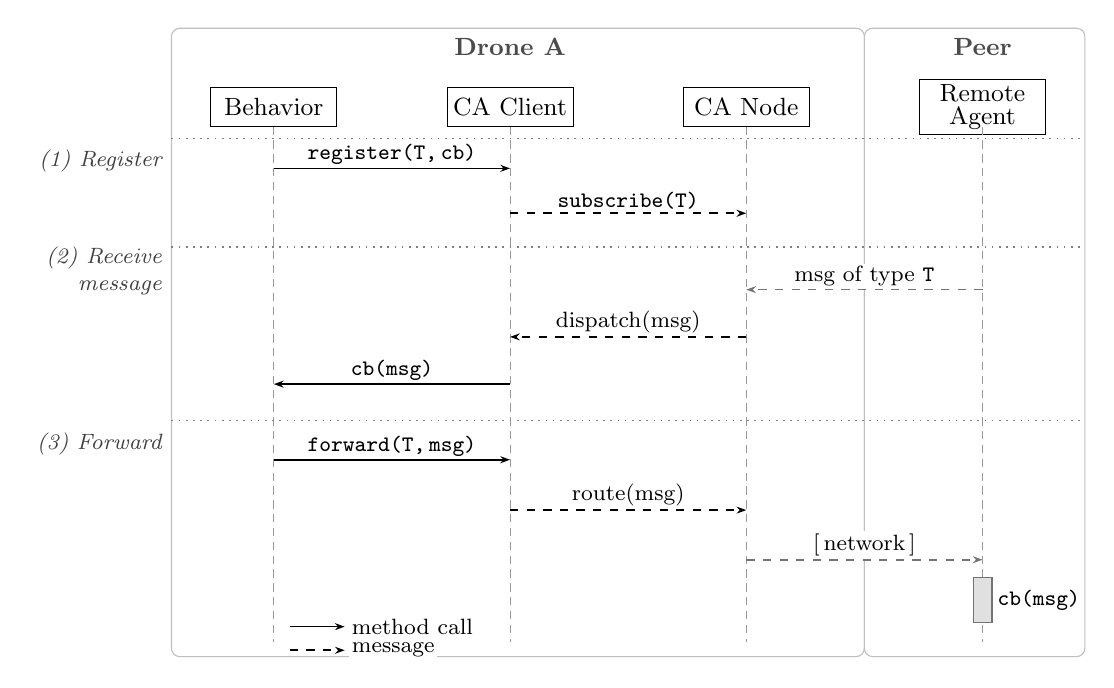
\begin{tikzpicture}[
  font=\small,
  box/.style={draw, fill=white, rectangle, minimum width=1.6cm,
              minimum height=0.50cm, align=center, inner sep=2pt},
  ll/.style={densely dashed, black!40},
  arr/.style={-{Stealth[length=3.5pt,width=2.5pt]}, semithick},
  marr/.style={-{Stealth[length=3.5pt,width=2.5pt]}, semithick, dashed},
  narr/.style={-{Stealth[length=3.5pt,width=2.5pt]}, semithick, dashed, black!55},
  lbl/.style={font=\footnotesize, fill=white, inner sep=1pt},
  sep/.style={dotted, black!50, semithick},
  phase/.style={font=\footnotesize\itshape, black!75},
]
  \def\xA{0}    % Behavior
  \def\xB{3.0}  % CA Client
  \def\xC{6.0}  % CA Node
  \def\xD{9.0}  % Remote Agent

  % --- Participant boxes ---
  \node[box] at (\xA,0) (pA) {Behavior};
  \node[box] at (\xB,0) (pB) {CA Client};
  \node[box] at (\xC,0) (pC) {CA Node};
  \node[box] at (\xD,0) (pD) {\shortstack{Remote\\[-1pt]Agent}};

  % --- Lifelines ---
  \foreach \x in {\xA,\xB,\xC,\xD}
    \draw[ll] (\x,-0.25) -- (\x,-6.8);

  % --- Grouping outlines ---
  \draw[rounded corners=3pt, black!25]
    (-1.3,1.0) rectangle (7.5,-6.98);
  \node[font=\small\bfseries, text=black!70, anchor=north]
    at ({(\xA+\xC)/2}, 1.0) {Drone A};
  \draw[rounded corners=3pt, black!25]
    (7.5,1.0) rectangle (10.3,-6.98);
  \node[font=\small\bfseries, text=black!70, anchor=north]
    at (\xD, 1.0) {Peer};

  % ======== (1) Register ========
  \draw[sep] (-1.3,-0.40) -- (10.3,-0.40);
  \node[phase, anchor=east] at (-1.3,-0.68) {(1) Register};

  \draw[arr] (\xA,-0.78) -- (\xB,-0.78)
    node[lbl, above, midway] {\texttt{register(T,\,cb)}};
  \draw[marr] (\xB,-1.35) -- (\xC,-1.35)
    node[lbl, above, midway] {\texttt{subscribe(T)}};

  % ======== (2) Receive message ========
  \draw[sep] (-1.3,-1.78) -- (10.3,-1.78);
  \node[phase, anchor=east, align=right] at (-1.3,-2.08) {(2) Receive\\ message};

  \draw[narr] (\xD,-2.32) -- (\xC,-2.32)
    node[lbl, above, midway, text=black] {msg of type \texttt{T}};
  \draw[marr]  (\xC,-2.92) -- (\xB,-2.92)
    node[lbl, above, midway] {dispatch(msg)};
  \draw[arr]  (\xB,-3.52) -- (\xA,-3.52)
    node[lbl, above, midway] {\texttt{cb(msg)}};

  % ======== (3) Forward ========
  \draw[sep] (-1.3,-3.98) -- (10.3,-3.98);
  \node[phase, anchor=east] at (-1.3,-4.28) {(3) Forward};

  \draw[arr] (\xA,-4.48) -- (\xB,-4.48)
    node[lbl, above, midway] {\texttt{forward(T,\,msg)}};
  \draw[marr] (\xB,-5.12) -- (\xC,-5.12)
    node[lbl, above, midway] {route(msg)};
  \draw[narr] (\xC,-5.75) -- (\xD,-5.75)
    node[lbl, above, midway, text=black] {[\,network\,]};

  % Activation bar on peer lifeline
  \fill[black!12] (\xD-0.12,-5.98) rectangle (\xD+0.12,-6.55);
  \draw[black!55] (\xD-0.12,-5.98) rectangle (\xD+0.12,-6.55);
  \node[lbl, right] at (\xD+0.15,-6.27) {\texttt{cb(msg)}};

  % --- Legend ---
  \draw[arr]  (0.20,-6.60) -- (0.90,-6.60);
  \node[lbl, anchor=west] at (0.95,-6.60) {method call};
  \draw[marr] (0.20,-6.90) -- (0.90,-6.90);
  \node[lbl, anchor=west] at (0.95,-6.90) {message};

\end{tikzpicture}
\caption{CA Gateway message flow. Solid arrows denote method invocations (Behavior--CA Client); dashed arrows denote messages (CA Client--CA Node--Remote Agent). \textit{(1) Register}: a behavior declares callback \texttt{cb} for modelet type \texttt{T}; the CA Client subscribes at the node level. \textit{(2) Receive message}: when a peer sends a modelet of type \texttt{T}, the CA Node dispatches it to the CA Client, which invokes \texttt{cb}. \textit{(3) Forward}: a behavior calls \texttt{forward}; the CA Node serialises and routes the modelet to all registered peers. In all cases the behavior has no knowledge of peer addresses or network topology.}
\label{fig:gateway}
\end{figure}

Compared to direct use of ROS~2 cross-namespace topics, the CA Gateway operates at a higher level of abstraction. Raw DDS communication requires per-message-type topic definitions, static publisher--subscriber wiring, and explicit reconnection upon fleet reconfiguration. Consulting the ROS~2 graph at runtime to discover active nodes also incurs repeated query overhead that grows with fleet size. The CA Gateway Client abstracts this to two fleet-size-agnostic calls---\textit{register} and \textit{forward}---applicable uniformly across coordination protocols without per-protocol wiring; behavior code is identical in simulation (shared machine) and field deployment (Wi-Fi network). Table~\ref{tab:gateway_vs_dds} summarises the key differences.

\begin{table}[tbh]
\caption{CA Gateway vs.\ direct ROS~2 DDS cross-namespace communication.}
\label{tab:gateway_vs_dds}
\centering
\renewcommand{\arraystretch}{1.2}
\begin{tabular}{p{3.2cm}p{4.0cm}p{4.0cm}}
\hline
\textbf{Dimension} & \textbf{CA Gateway} & \textbf{Raw ROS~2 DDS} \\
\hline
Discovery overhead & Peer registry resolved once at send time & Graph queried per message type at runtime \\
Naming coupling & Typed registry; no topic names in behavior code & Per-message-type topic names hard-coded \\
Transport flexibility & Backend swappable (DDS, Zenoh, MQTT) & Tied to DDS \\
Fleet reconfiguration & Handled automatically by CA Gateway node & Explicit publisher/subscriber rewiring required \\
\hline
\end{tabular}
\end{table}

\section{CA Gateway node}

The \code{CA\_Gateway} node (package \code{as2\_ca}) is the per-drone communication hub that owns all inter-agent traffic. It continuously scans the active network, creates forwarding channels to newly discovered peers, and prunes channels for peers that have disappeared. This scan provides both runtime peer discovery and implicit failure detection: a crashed or disconnected drone ceases to be reachable within one discovery cycle, and its channel is automatically removed. Concretely, it performs three roles:

\begin{enumerate}
  \item \textbf{Peer discovery.} A one-second timer scans the live ROS~2 topic graph for topics whose name ends in \code{/gateway\_in}. Each newly found topic is added to an internal map of peer publishers; publishers whose topics have no subscribers are pruned. No prior knowledge of the fleet size is needed, and dynamic joins and departures are handled automatically, implementing the Swarm Size Awareness requirement IT-FR-028 from D7.2.

\begin{lstlisting}[language=C++, style=cppcolors,caption={Peer discovery in CA\_Gateway (simplified)}]
void CA_Gateway::check_peers()
{
  const std::string suffix = "/" + std::string(INCOMING_TOPIC_SUFFIX);
  auto topics = this->get_topic_names_and_types();
  for (auto & [name, types] : topics) {
    if (name ends with suffix && name != own_incoming_topic) {
      std::string peer_id = strip_prefix_and_suffix(name);
      if (not already known)
        create publisher to name and remember peer_id;
    }
  }
  prune peers with no subscribers;
}
\end{lstlisting}

  \item \textbf{Outbound forwarding.} The gateway subscribes to its drone's \code{gateway\_out} topic. When a behavior publishes a \code{LocalGenericMessage} there, the gateway serialises it into an \code{InterAgentMessage} and publishes it to the \code{gateway\_in} topic of each named recipient---using the publisher map built by peer discovery. This corresponds to step~(3) in Figure~\ref{fig:gateway}: the behavior calls \texttt{forward} on the CA Client, which publishes to \code{gateway\_out}; the CA Node then fans the packet out to all named peers.

  \item \textbf{Inbound demultiplexing.} The gateway subscribes to its own \code{/\{namespace\}/gateway\_in} topic. When an \code{InterAgentMessage} arrives from a peer, it looks up the registered handler for the message's \code{type} tag and forwards a \code{LocalGenericMessage} to the corresponding local topic, as depicted in step~(2) of Figure~\ref{fig:gateway}. This implements the D7.3 requirement to \emph{distribute incoming modelets to the corresponding cognitive modules}, closing the delivery loop from remote sender to local behavior callback.
\end{enumerate}

Figures~\ref{fig:gw_inbound} and~\ref{fig:gw_outbound} illustrate each path in detail.

% ------------------------------------------------------------------
% Figure: Inbound demultiplexing
% ------------------------------------------------------------------
\begin{figure}[tbh]
\centering
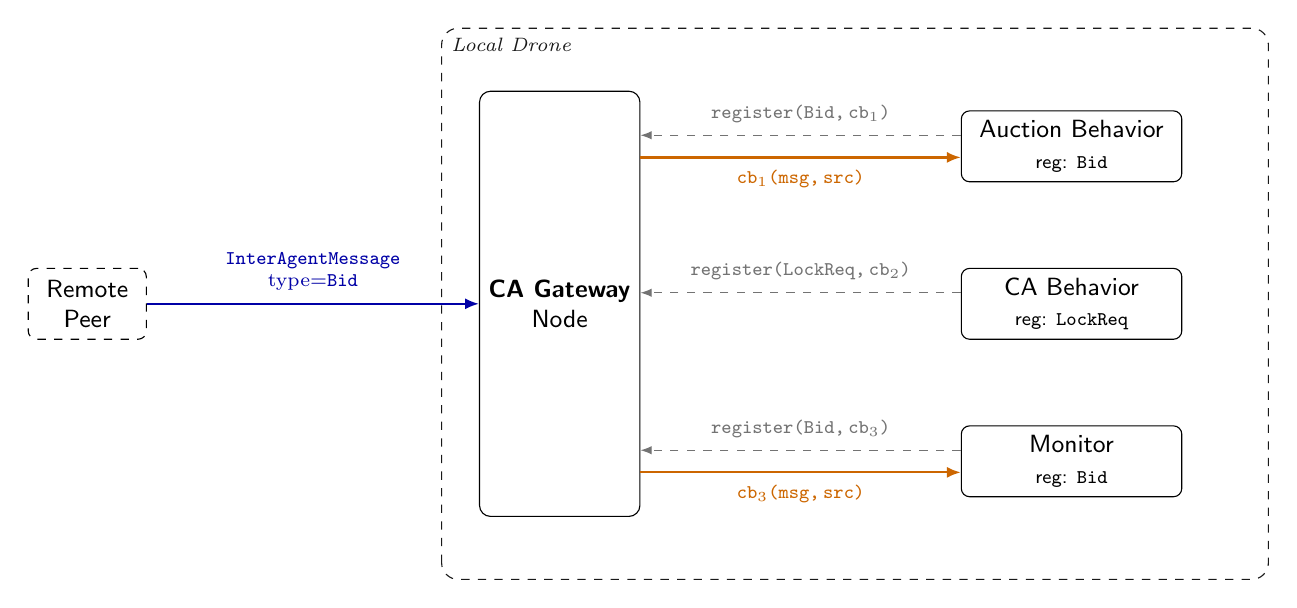
\begin{tikzpicture}[
  cbox/.style  = {draw, rounded corners=3pt, minimum width=2.8cm,
                  minimum height=0.9cm, align=center,
                  font=\small\sffamily, fill=white},
  gwbox/.style = {draw, rounded corners=4pt, minimum width=2.0cm,
                  minimum height=5.4cm, align=center,
                  font=\small\sffamily, fill=white},
  pbox/.style  = {draw, dashed, rounded corners=3pt, minimum width=1.5cm,
                  minimum height=0.9cm, align=center,
                  font=\small\sffamily, fill=white},
  regarr/.style= {-{Latex[length=4pt,width=3pt]}, thin, black!55, dashed},
  disarr/.style= {-{Latex[length=5pt,width=4pt]}, thick, orange!80!black},
  inarr/.style = {-{Latex[length=5pt,width=4pt]}, thick, blue!65!black},
  rlbl/.style  = {font=\scriptsize, align=center, text=black!55},
  dlbl/.style  = {font=\scriptsize, align=center, text=orange!80!black},
  ilbl/.style  = {font=\scriptsize, align=center, text=blue!65!black},
]

\node[pbox]  (peer) at (0, 0)     {Remote\\Peer};
\node[gwbox] (gw)   at (6.0, 0)   {\textbf{CA Gateway}\\Node};
\node[cbox]  (b1)   at (12.5,  2.0)
  {Auction Behavior\\{\scriptsize reg: \texttt{Bid}}};
\node[cbox]  (b2)   at (12.5,  0.0)
  {CA Behavior\\{\scriptsize reg: \texttt{LockReq}}};
\node[cbox]  (b3)   at (12.5, -2.0)
  {Monitor\\{\scriptsize reg: \texttt{Bid}}};

\draw[black!90, dashed, rounded corners=6pt]
  (4.5,-3.5) rectangle (15.0,3.5);
\node[black!90, font=\scriptsize\itshape, anchor=north west]
  at (4.5,3.5) {Local Drone};

% Inbound message
\draw[inarr] (peer.east)
  -- node[ilbl, above=1pt] {\texttt{InterAgentMessage}\\type=\texttt{Bid}}
  (gw.west);

% Registration arrows (behavior → gateway)
\draw[regarr] ([yshift=4pt]b1.west)
  -- node[rlbl, above=1pt] {\texttt{register(Bid,\,cb}$_1$\texttt{)}}
  ([yshift=4pt]gw.east|-b1);
\draw[regarr] ([yshift=4pt]b2.west)
  -- node[rlbl, above=1pt] {\texttt{register(LockReq,\,cb}$_2$\texttt{)}}
  ([yshift=4pt]gw.east|-b2);
\draw[regarr] ([yshift=4pt]b3.west)
  -- node[rlbl, above=1pt] {\texttt{register(Bid,\,cb}$_3$\texttt{)}}
  ([yshift=4pt]gw.east|-b3);

% Dispatch arrows (gateway → Bid-registered behaviors only)
\draw[disarr] ([yshift=-4pt]gw.east|-b1)
  -- node[dlbl, below=1pt] {\texttt{cb}$_1$\texttt{(msg,\,src)}}
  ([yshift=-4pt]b1.west);
\draw[disarr] ([yshift=-4pt]gw.east|-b3)
  -- node[dlbl, below=1pt] {\texttt{cb}$_3$\texttt{(msg,\,src)}}
  ([yshift=-4pt]b3.west);

\end{tikzpicture}
\caption{Inbound demultiplexing. Each behavior registers a typed callback with the
CA~Gateway (grey dashed arrows). When a \texttt{Bid} \texttt{InterAgentMessage}
arrives from a remote peer (blue), the gateway dispatches it only to the two behaviors
registered for type \texttt{Bid} (orange). The behavior registered for a different
type (\texttt{LockReq}) receives no dispatch.}
\label{fig:gw_inbound}
\end{figure}

% ------------------------------------------------------------------
% Figure: Outbound forwarding
% ------------------------------------------------------------------
\begin{figure}[tbh]
\centering
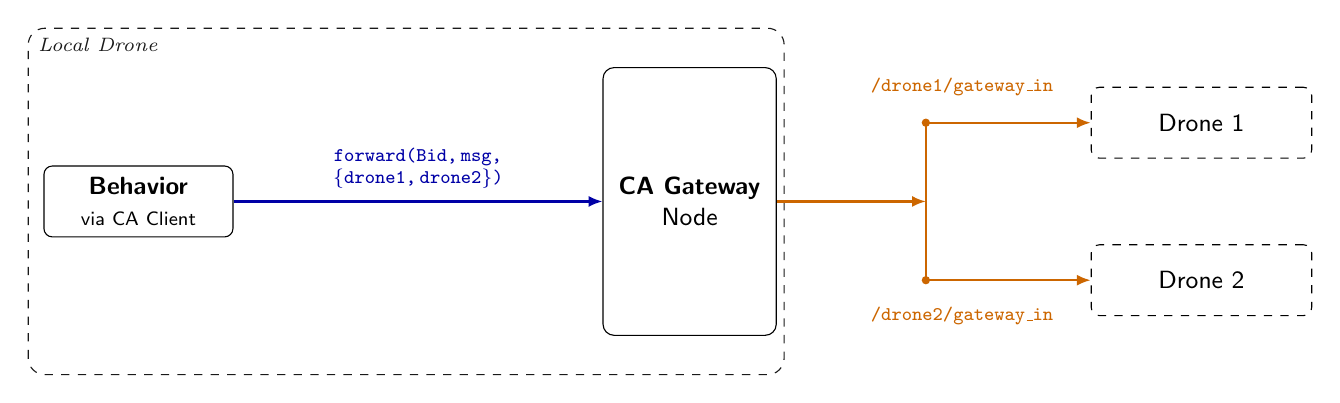
\begin{tikzpicture}[
  cbox/.style  = {draw, rounded corners=3pt, minimum width=2.4cm,
                  minimum height=0.9cm, align=center,
                  font=\small\sffamily, fill=white},
  gwbox/.style = {draw, rounded corners=4pt, minimum width=2.2cm,
                  minimum height=3.4cm, align=center,
                  font=\small\sffamily, fill=white},
  pbox/.style  = {draw, dashed, rounded corners=3pt, minimum width=2.8cm,
                  minimum height=0.9cm, align=center,
                  font=\small\sffamily, fill=white},
  oarr/.style  = {-{Latex[length=5pt,width=4pt]}, thick, blue!65!black},
  farr/.style  = {-{Latex[length=5pt,width=4pt]}, thick, orange!80!black},
  olbl/.style  = {font=\scriptsize, align=center, text=blue!65!black},
  flbl/.style  = {font=\scriptsize, align=center, text=orange!80!black},
]

\node[cbox]  (beh) at (0, 0)
  {\textbf{Behavior}\\{\scriptsize via CA~Client}};
\node[gwbox] (gw)  at (7.0, 0) {\textbf{CA Gateway}\\Node};
\node[pbox]  (p1)  at (13.5,  1.0)
  {Drone~1};
\node[pbox]  (p2)  at (13.5, -1.0)
  {Drone~2};

\draw[black!90, dashed, rounded corners=6pt]
  (-1.4,-2.2) rectangle (8.2,2.2);
\node[black!90, font=\scriptsize\itshape, anchor=north west]
  at (-1.4,2.2) {Local Drone};


% forward() call: behavior supplies peer names, not topic paths
\draw[oarr] (beh.east)
  -- node[olbl, above=1pt]
       {\texttt{forward(Bid,\,msg,}\\%
        \texttt{\{drone1,\,drone2\})}}
  (gw.west);

% Fan-out: horizontal stem → vertical bus → horizontal arrows to each peer
\coordinate (branch) at (10.0, 0);
\draw[farr] (gw.east) -- (branch);
\draw[thick, orange!80!black] (branch) -- (branch |- p1);
\draw[thick, orange!80!black] (branch) -- (branch |- p2);
\draw[farr] (branch |- p1)
  -- node[flbl, above=13pt, left=-20pt] {\texttt{/drone1/gateway\_in}}
  (p1.west);
\draw[farr] (branch |- p2)
  -- node[flbl, below=13pt, left=-20pt] {\texttt{/drone2/gateway\_in}}
  (p2.west);
\fill[orange!80!black] (branch |- p1) circle (1.5pt);
\fill[orange!80!black] (branch |- p2) circle (1.5pt);

\end{tikzpicture}
\caption{Outbound forwarding. The behavior calls \texttt{forward} with a modelet type,
a payload, and a list of peer \emph{names}---it has no knowledge of how those peers
are addressed on the network. The CA~Gateway resolves each name to the corresponding
\texttt{gateway\_in} publisher (maintained by the peer-discovery timer) and fans the
\texttt{InterAgentMessage} out to every named peer. The behavior's code is therefore
identical regardless of fleet size or network topology.}
\label{fig:gw_outbound}
\end{figure}

\section{Message types: the modelet vocabulary}

The message types that flow through the gateway are the concrete ROS~2 representation of the modelets described in D7.3. Added to \code{as2\_msgs}, they directly address one of the core challenges identified in D7.3~\cite{CORESENSE-D73}: ensuring that communication between agents is not merely syntactically valid but \emph{semantically intelligible}---that both sender and receiver attach the same meaning to the transmitted information.

D7.3 solves this by requiring that agents share a common modelet vocabulary: a set of agreed-upon data structures whose interpretation is identical across the fleet. \code{LocalGenericMessage} and \code{InterAgentMessage} are the envelopes that carry this vocabulary. Because every agent in the fleet uses the same \code{as2\_msgs} message definitions, the shared semantics are enforced at compile time: a \code{Bid} modelet published by one drone is guaranteed to be parsed identically by any other drone running the same software stack. These two message types are therefore not merely transport containers---they are the embodiment of the common understanding that D7.3 requires for effective inter-agent communication.

\subsection{Transport envelope}

\begin{description}
  \item[\tcode{InterAgentMessage}] The carrier for any typed modelet on the inter-drone channel. It contains a \code{sender} field (the originating drone namespace), a \code{type} tag identifying the modelet kind, and a raw \code{uint8[]} \code{data} field carrying the serialised ROS~2 payload. This message type represents the \emph{shared semantic substrate} of the multi-agent system: its \code{type} tag and \code{data} encoding are governed by the common \code{as2\_msgs} vocabulary, ensuring that any agent capable of receiving a message of a given type can unambiguously interpret its content.

  \item[\tcode{LocalGenericMessage}] The intra-agent dual of \code{InterAgentMessage}, used between a behavior and its drone's gateway. It carries a list of \code{agents} (target recipients or original senders), a \code{type} tag, and the same raw \code{data} field. It decouples the behavior from the transport layer: the behavior speaks the shared modelet vocabulary without needing to know how the gateway addresses or routes the message to peers.
\end{description}

The gateway translates between these two representations: outbound \code{LocalGenericMessage} messages from behaviors are wrapped into \code{InterAgentMessage} and routed to peers; inbound \code{InterAgentMessage} packets from peers are unwrapped and delivered as \\ \code{LocalGenericMessage} to the registered local handler. In this way, the shared modelet vocabulary defined in D7.3 is preserved end-to-end without any loss of semantic fidelity during transport.

\subsection{Auction modelets}

These messages implement the modelets for the \emph{auctions} collective model (D7.3 Table~5.1).

\begin{description}
  \item[\tcode{AuctionItem}] A single item to be auctioned. Carries a \code{name} string, a \code{features} float64 array, and a \code{feature\_names} string array, encoding any quantity relevant to cost computation (target coordinates, priority weights, etc.).
  \item[\tcode{AuctionItemArray}] A container for multiple \code{AuctionItem} messages, also carrying the name of the item-type plugin to use for cost computation.
  \item[\tcode{StartAuction}] Sent by the auctioneer to all participants; carries the item list and the set of bidder namespaces.
  \item[\tcode{Bid}] The core auction modelet---the \emph{bid of each individual agent} of D7.3 Table~5.1. It carries the \code{name} array of the items the agent has evaluated and an \code{amounts} float64 array of the corresponding costs.
\end{description}

\subsection{Path-lock modelets}

These messages implement the modelets for the \emph{consensus} collective models: the individual path plans and the lock grants that encode the collectively agreed access schedule.

\begin{description}
  \item[\tcode{PoseStampedWithID}] A \code{geometry\_msgs/PoseStamped} augmented with a string \code{id}, used to identify waypoints in a planned path.
  \item[\tcode{CAPathLockRequest}] Sent by a drone requesting exclusive access to a path corridor. Contains the \code{requester\_id}, a monotonically increasing \code{req\_id}, and the \code{path} as a \\ \code{PoseStampedWithID} array.
  \item[\tcode{CAPathLockGrant}] Sent by each peer to acknowledge a lock request. Contains the \code{granter\_id}, the \code{requester\_id}, and the matching \code{req\_id}. Receiving a grant from every peer constitutes the consensus that the requesting drone may proceed.
  \item[\tcode{CAPathLockRelease}] Sent by a drone on finishing a locked corridor, allowing deferred peers to proceed.
\end{description}

\section{CA Gateway Client}

The CA Gateway Client is simultaneously the \emph{brownfield integration point} of the collective awareness layer and the \emph{behavior-side enforcement point of the participation contract}. As an integration point, it lets Aerostack2 gain inter-agent communication capability without modifying a single line of existing component code: existing behaviors, platform drivers, and mission scripts are entirely unaware of its existence, and adding collective awareness is purely additive. As a contract enforcement point, instantiating a \code{CAGatewayClient} is the \emph{only} way for a behavior to register modelet handlers or send inter-agent modelets, there is no side-channel. Any behavior that uses the API therefore automatically satisfies the registration and routing obligations of the contract; any behavior that does not use it cannot accidentally or inadvertently participate in a collective process. The CA Client thus makes compliance with the contract the path of least resistance: a new behavior instantiates it and calls two methods, and the drone is immediately capable of correct, contract-compliant inter-agent modelet exchange.

Behaviors do not interact with the gateway node directly. Instead, each behavior instantiates a \code{CAGatewayClient} (header-only, \code{as2\_ca/ca\_gateway\_client.hpp}), a lightweight library that wraps the gateway's registration service, the \code{gateway\_out} publisher, and type-parametric deserialisation into a clean, type-safe API. It exposes two operations that directly mirror the sequence diagram in Figure~\ref{fig:gateway}:

\begin{itemize}
  \item \textbf{\textit{register}} declares interest in a modelet type and provides a callback invoked on arrival (step 1 in Figure~\ref{fig:gateway}).
  \item \textbf{\textit{forward}} sends a typed modelet to a named set of peers (step 3 in Figure~\ref{fig:gateway}).
\end{itemize}

From the behavior's perspective, the experience is deliberately analogous to native ROS~2 publish--subscribe: \textit{register} is the inter-agent equivalent of creating a subscription with a callback, and \textit{forward} is the equivalent of publishing to a topic. The key difference is that the CA Client handles addressing, fleet discovery, and cross-agent routing transparently---the behavior specifies only the modelet type and the target agent namespaces, with no knowledge of how those agents are reached. Inter-agent communication through the CA Node is therefore \emph{transparent to the behavior author}: writing a collective behavior feels almost identical to writing a standard single-drone behavior that publishes and subscribes to local ROS~2 topics.

From the behavior's perspective, peer addresses, network topology, and transport details are completely hidden.

\textbf{Registering a modelet handler} announces to the gateway which message type the behavior handles under a given tag, and provides the callback to invoke on receipt:

\begin{lstlisting}[language=C++, style=cppcolors,caption={Registering a typed modelet handler}]
client_.register_module<as2_msgs::msg::Bid>(
  "bid",               // type tag
  "auction_behavior",  // module name
  [this](const as2_msgs::msg::Bid & msg, const std::string & sender) {
    auction_plugin_->on_bid_received(msg, sender);
  });
\end{lstlisting}

\textbf{Sending a modelet} serialises a typed ROS~2 message and routes it to a named list of peers:

\begin{lstlisting}[language=C++, style=cppcolors,caption={Forwarding a typed modelet to a list of peers}]
client_.forward_IA_msg<as2_msgs::msg::Bid>(bid, "bid", participants_);
\end{lstlisting}

Internally, \code{forward\_IA\_msg} uses \code{rclcpp::Serialization<T>} to pack the message bytes into a \code{LocalGenericMessage} and publishes it to \code{gateway\_out}. The CA Gateway node then routes the packet to each named peer's \code{gateway\_in} topic, following the path shown in step 3 of Figure~\ref{fig:gateway}.

This two-level design---gateway node for transport, client library for type safety---cleanly separates the communication concern (routing, addressing, fleet management) from the application concern (which modelet type to send, what to do on receipt), mirroring the layered structure of the Communication Interface subsystem in D7.3.

%%%%%%%%%%%%%%%%%%%%%%%%%%%%%%%%%%%%%%%%%%%%%%%%%%%%%%%%%%%%%%%%%%%%%%%%%%%%%

\chapter{Knowledge Base Interface}
\label{ch:kb}

The knowledge base used for this testbed (\code{knowledge\_core} \cite{knowledge_core}) stores and reasons over RDF triples and emits events when registered patterns are satisfied. It is the persistent, semantic integration layer that connects individual agent observations to collective reasoning: a fact asserted by one drone's behavior can trigger a mission-level reaction in another drone's Python monitor, implementing the information sharing requirement IT-FR-027 from D7.2. Two complementary interfaces connect Aerostack2 to it.

\section{C++ KBInterface}

\code{knowledge\_core} is the CORESENSE knowledge base server: a ROS~2 node that stores and reasons over RDF triples and exposes three interfaces to other nodes: a topic pair for asserting and retracting facts (\code{kb/add\_fact}, \code{kb/remove\_fact}), a service for clause-based queries (\code{kb/query}), and an event-notification mechanism that publishes to registered topics whenever a declared triple pattern is satisfied. It acts as the shared, persistent memory an agent operating in the multi-drone system: any agent can write facts about its own state or collective decisions, and any other agent, or mission-level script, can query or react to those facts without polling. Because \code{knowledge\_core} is a separate ROS~2 node, behaviors interact with it through the interfaces below without being coupled to its internal implementation.

The \code{as2::KBInterface} class (header \code{as2\_core/kb\_interface.hpp}) provides behaviors with a synchronous-style API for asserting, retracting, and querying facts:

\begin{description}
  \item[\tcode{add\_fact(subj, pred, obj)}] Publishes a space-separated triple to the \code{kb/add\_fact} topic.
  \item[\tcode{remove\_fact(subj, pred, obj)}] Publishes to \code{kb/remove\_fact}.
  \item[\tcode{query\_kb(clauses, variables)}] Calls the \code{kb/query} service and returns the first binding map.
  \item[\tcode{query\_kb\_all(clauses, variables)}] Returns all binding maps.
  \item[\tcode{register\_event\_handler(topic, handler)}] Subscribes to a KB event topic and invokes a callback on each trigger.
\end{description}

Service calls are handled on a dedicated background thread backed by a \code{SingleThreadedExecutor}, so \code{query\_kb} and \code{query\_kb\_all} can block safely from inside a ROS~2 callback without re-entering the calling node's executor. This allows behaviors to treat knowledge-base queries as synchronous operations even though they cross node boundaries.

\section{Python KB Monitor}

This monitor handles mission-level logic, deciding when to trigger replanning, when to resume execution, and when to ground a failing drone. The \code{as2\_python\_api.kb\_monitor} sub-package implements this layer as a single \code{KBMonitorNode}: a ROS~2 node that subscribes to \code{knowledge\_core} events and dispatches them to registered Python handler functions. Rather than polling the knowledge base, the monitor declares which RDF triple patterns are of interest; \code{knowledge\_core} notifies the node whenever matching facts appear, and the node invokes the corresponding handler. This event-driven design decouples mission scripts from behavior timing: behaviors and mission scripts interact solely through the shared KB vocabulary, with no direct call dependencies between them.

\textbf{Configuration and launch.} The node is configured via a JSON file and launched by \\ \code{launch\_kb\_monitor.py}, a CLI entry point that accepts the config path and a \code{drone\_namespace} argument. The launcher parses the JSON, instantiates a \code{KBMonitorNode}, calls \code{register\_handler} once per entry, and spins the node under a \code{MultiThreadedExecutor}. Each JSON entry specifies:

\begin{itemize}
  \item \code{id} --- a unique identifier for the handler;
  \item \code{patterns} --- RDF triple patterns with \code{?}-prefixed variables;
  \item \code{one\_shot} --- whether to remove the handler after the first trigger;
  \item \code{models} --- optional list of KB models to watch (\code{[]} means all);
  \item \code{func} --- the Python module path and function name to invoke on each trigger.
\end{itemize}

\begin{lstlisting}[language=Python, style=pycolors,caption={KB Monitor JSON configuration file}]
{
  "kb_namespace": "kb",
  "handlers": [
    {
      "id": "assignment_done",
      "patterns": ["?drone is_assigned_to ?target"],
      "one_shot": false,
      "models": [],
      "func": {
        "path": "/path/to/handlers.py",
        "name": "handlers_module",
        "func_name": "on_assignment"
      }
    }
  ]
}
\end{lstlisting}

\begin{itemize}
  \item \textbf{Error modes}: if a handler raises an exception, it is logged and that invocation is dropped without crashing the node.
  \item \textbf{Reentrancy}: handlers should be idempotent or use \code{one\_shot} when the pattern should fire exactly once, since publishing a \code{MissionUpdate} from a handler may itself produce KB events.

  \item \textbf{Handler contract.} Each handler is a plain Python function with signature \code{handler(bindings, ctx)}. \code{bindings} is a list of variable-binding dicts published by \code{knowledge\_core} (e.g.\ \code{[\{'drone': 'drone0', 'target': 'T1'\}]}). \code{ctx} is a \code{KBHandlerContext} that exposes:

    \begin{itemize}
      \item \code{query(patterns, vars)} --- synchronous KB query, safe to call from callbacks;
      \item \code{add\_fact(triple)} / \code{remove\_fact(triple)} --- assert or retract KB facts;
      \item \code{publish\_mission\_update(msg)} --- publish a \code{MissionUpdate} to the mission interpreter;
      \item \code{mission\_status} and \code{pose} --- latest cached values, updated automatically.
    \end{itemize}

    Handler functions impose no base-class requirement and can live in any importable Python module referenced by the JSON config.
    
    \begin{lstlisting}[language=Python, style=pycolors,caption={KB event handler function}]
    from as2_msgs.msg import MissionUpdate
    
    def on_assignment(bindings, ctx):
        for b in bindings:
            msg = MissionUpdate()
            msg.drone_id = b['drone']
            msg.action = MissionUpdate.RESUME
            msg.target = b['target']
            ctx.publish_mission_update(msg)
    \end{lstlisting}

\end{itemize}


%%%%%%%%%%%%%%%%%%%%%%%%%%%%%%%%%%%%%%%%%%%%%%%%%%%%%%%%%%%%%%%%%%%%%%%%%%%%%

\chapter{Auction Behavior}
\label{ch:auction}

\section{Overview: auctions as a collective model}

Task allocation in the inspection scenario is an instance of the \emph{auctions} collective model identified in D7.3: the auctioneer drone publishes a set of inspection targets (items), all participating drones simultaneously compute and broadcast their costs (bids), and each drone resolves conflicts locally until a stable assignment emerges. Because every agent adopts an honest stance---its bid reflects its actual cost to reach each target---this is a fair-division auction.

The \code{as2\_auction\_behavior} package implements this collective model as an Aerostack2 behavior server backed by two plugin hierarchies. The behavior uses three of the components described above:
\begin{itemize}
  \item the \textbf{CA Gateway} to distribute the item list and exchange bid modelets;
  \item the \textbf{State Interface} to read the drone's current pose for cost computation;
  \item the \textbf{KB Interface} to record the assignment as facts in the knowledge base.
\end{itemize}

This behavior satisfies D7.2 requirements IT-FR-002 (collaborative planning) and IT-FR-003 (system replanning): when a drone failure is detected and its targets become unallocated, the auctioneer triggers a new auction round over only the uncovered targets.

\section{Action interface}

The behavior exposes the \code{as2\_msgs/action/Auction} action. The goal specifies:
\begin{itemize}
  \item \code{name} --- a unique auction identifier;
  \item \code{elements} --- the \code{AuctionItem} modelets to allocate;
  \item \code{type} --- the auction strategy plugin (e.g.\ \code{greedy\_sequential});
  \item \code{bidders} --- the namespaces of all participating drones.
\end{itemize}
Feedback reports which items have been assigned so far; the result returns the complete assignment map.

\section{Plugin architecture}

\subsection{AuctionBehaviorPluginBase}

The abstract base class defines the engine interface:
\begin{itemize}
  \item \code{on\_activate(goal)} / \code{on\_deactivate()} --- lifecycle hooks;
  \item \code{on\_auction\_items\_received(msg, agent\_id)} --- called when the item-list modelet arrives from the auctioneer via the CA Gateway.
  \item \code{compute\_bid()} --- queries the State Interface for the information about the drone state, and calls the item plugin to generate a bid for a subset fo the available items.
  \item \code{update(bid, agent\_id)} --- integrates a peer's bid modelet and re-runs conflict resolution.
  \item \code{check\_convergence()} --- returns a boolean indicating when the auction has finished.
  \item \code{get\_global\_assignment()} --- returns the item$\to$winner map.
\end{itemize}

\subsection{AuctionItemPluginBase}

A second plugin type abstracts cost computation for a specific item kind. This separation keeps the auction strategy agnostic about item semantics. The \code{coordinate\_item} plugin computes Euclidean distance from the drone's current pose to a 3-D coordinate target.

\subsection{Greedy Sequential plugin}

The \code{greedy\_sequential} plugin implements the following protocol:

\begin{enumerate}
  \item On receiving the item list, compute costs for every item and broadcast a \code{Bid} modelet to all participants via the CA Gateway.
  \item On receiving a peer's \code{Bid} modelet, store it and run conflict resolution: assign each item to the agent with the lowest cost; break ties lexicographically by agent namespace.
  \item Declare convergence once a bid has been received from every participant (including self).
\end{enumerate}

Because every agent applies the same deterministic rule to the same set of bids, local and global assignments converge identically without additional communication rounds.

\section{Using the CA Gateway}

The auction behavior uses \code{CAGatewayClient} for all modelet exchange. On activation the behavior registers two handlers---one for incoming \code{StartAuction} modelets (auctioneer distributing the item list) and one for incoming \code{Bid} modelets (peers broadcasting their costs):

\begin{lstlisting}[language=C++, style=cppcolors,caption={Registering auction modelet handlers}]
client_.register_module<as2_msgs::msg::StartAuction>(
  "start_auction", "auction_behavior",
  [this](const as2_msgs::msg::StartAuction & msg, const std::string &) {
    auction_plugin_->on_auction_items_received(msg.items, msg.auctioneer);
  });

client_.register_module<as2_msgs::msg::Bid>(
  "bid", "auction_behavior",
  [this](const as2_msgs::msg::Bid & msg, const std::string & sender) {
    auction_plugin_->on_bid_received(msg, sender);
  });
\end{lstlisting}

The \code{register\_module} call is the inter-agent analogue of \code{create\_subscription}: both declare interest in a typed message and install a callback, but \code{register\_module} requires no topic address, covers all current and future peers automatically, and delivers the sender's namespace as a second argument. Figure~\ref{fig:register_vs_sub} illustrates the difference.

\begin{figure}[tbh]
\centering
\begin{minipage}[t]{0.47\linewidth}
\begin{lstlisting}[language=C++, style=cppcolors,
  title={Raw ROS~2 (one per peer)},
  basicstyle=\ttfamily\footnotesize]
using Bid = as2_msgs::msg::Bid;
// repeated for every peer:
bid_sub_ =
  node->create_subscription<Bid>(
    "/drone1/bids", 10,
    [this](const Bid & msg) {
      on_bid_received(msg, "drone1");
    });
\end{lstlisting}
\end{minipage}%
\hfill
\begin{minipage}[t]{0.47\linewidth}
\begin{lstlisting}[language=C++, style=cppcolors,
  title={CA Client (all peers)},
  basicstyle=\ttfamily\footnotesize]
using Bid = as2_msgs::msg::Bid;
// once for all peers:
client_.register_module<Bid>(
  "bid", "auction_behavior",
  [this](const Bid & msg,
         const std::string & src) {
    on_bid_received(msg, src);
  });
\end{lstlisting}
\end{minipage}
\caption{Comparison between a raw ROS~2 subscription and a CA Client registration for the same \code{Bid} message type. The ROS~2 approach requires one \code{create\_subscription} call per peer with a hard-coded topic name and sender identity; \code{register\_module} replaces all of them with a single call that receives the sender namespace dynamically via \code{src}.}
\label{fig:register_vs_sub}
\end{figure}

When \code{compute\_bid()} produces a cost vector, the plugin broadcasts it to all bidders:

\begin{lstlisting}[language=C++, style=cppcolors,caption={Broadcasting the bid modelet}]
client_.forward_IA_msg<as2_msgs::msg::Bid>(bid, "bid", bidders_);
\end{lstlisting}

Figure~\ref{fig:ca_gateway_auction} traces the complete CA Gateway message flow for a two-drone auction interaction, covering registration, item announcement, bid exchange, and convergence.

\begin{figure}[tbh]
\centering
\resizebox{\textwidth}{!}{%
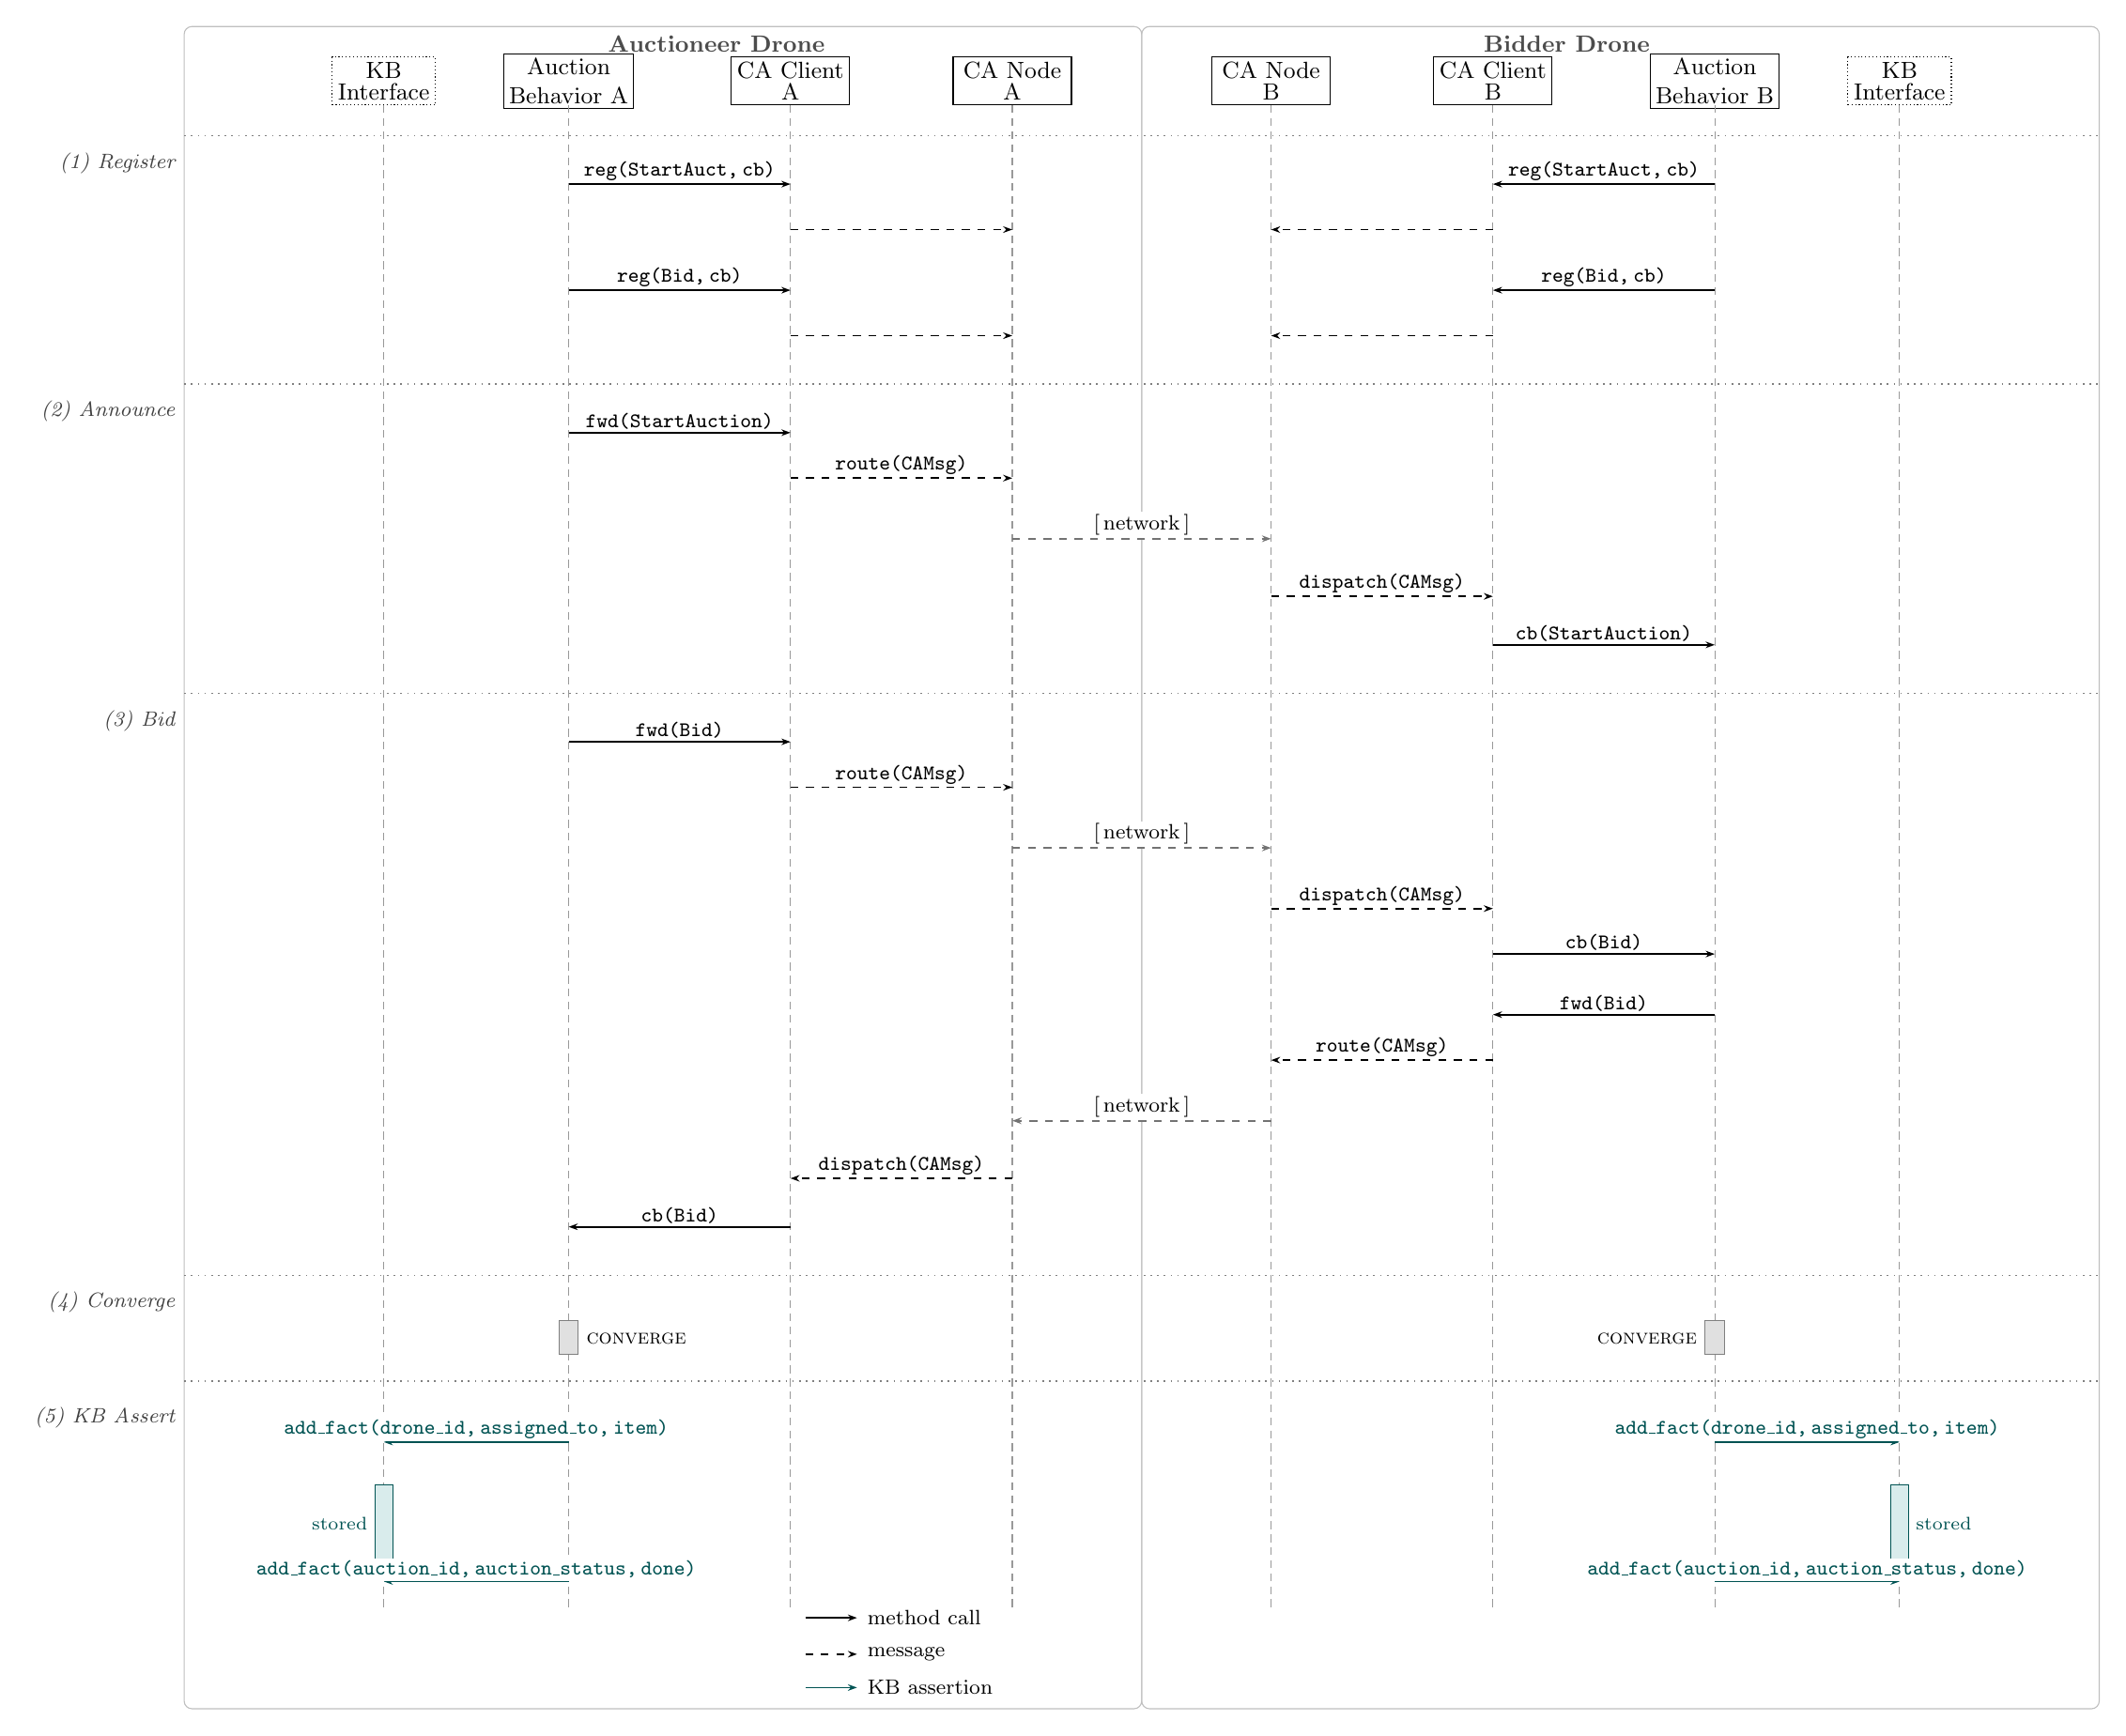
\begin{tikzpicture}[yscale=0.82,
  font=\small,
  box/.style={draw, fill=white, rectangle, minimum width=1.6cm,
              minimum height=0.52cm, align=center, inner sep=2pt},
  kbbox/.style={draw, fill=white, rectangle, minimum width=1.4cm,
              minimum height=0.52cm, align=center, inner sep=2pt, densely dotted},
  ll/.style={densely dashed, black!40},
  arr/.style={-{Stealth[length=3.5pt,width=2.5pt]}, semithick},
  marr/.style={-{Stealth[length=3.5pt,width=2.5pt]}, semithick, dashed},
  narr/.style={-{Stealth[length=3.5pt,width=2.5pt]}, semithick, dashed, black!55},
  kbarr/.style={-{Stealth[length=3.5pt,width=2.5pt]}, semithick, teal!65!black},
  lbl/.style={font=\footnotesize, fill=white, inner sep=1pt},
  sep/.style={dotted, black!50, semithick},
  phase/.style={font=\footnotesize\itshape, black!75},
]

  \def\xKBA{-2.5}  % KB Interface (Auctioneer Drone)
  \def\xA{0}       % Auctioneer behavior
  \def\xEA{3.0}    % CA Client A
  \def\xB{6.0}     % CA Node A
  \def\xC{9.5}     % CA Node B
  \def\xEB{12.5}   % CA Client B
  \def\xD{15.5}    % Bidder behavior
  \def\xKBB{18.0}  % KB Interface (Bidder Drone)

  % --- Participant boxes ---
  \node[kbbox] at (\xKBA, .3) {\shortstack{KB\\[-1pt]Interface}};
  \node[box]   at (\xA,.3)   {Auction \\ Behavior A};
  \node[box]   at (\xEA,.3)  {\shortstack{CA Client\\[-1pt]A}};
  \node[box]   at (\xB,.3)   {\shortstack{CA Node\\[-1pt]A}};
  \node[box]   at (\xC,.3)   {\shortstack{CA Node\\[-1pt]B}};
  \node[box]   at (\xEB,.3)  {\shortstack{CA Client\\[-1pt]B}};
  \node[box]   at (\xD,.3)   {Auction \\ Behavior B};
  \node[kbbox] at (\xKBB,.3) {\shortstack{KB\\[-1pt]Interface}};

  % --- Lifelines ---
  \foreach \x in {\xKBA,\xA,\xEA,\xB,\xC,\xEB,\xD,\xKBB}
    \draw[ll] (\x,-0.1) -- (\x,-24.90);

  % --- Group outlines ---
  \draw[rounded corners=3pt, black!25]
    (-5.2, 1.2) rectangle (7.75,-26.55);
  \node[font=\small\bfseries, text=black!70, anchor=north]
    at (2.0, 1.2) {Auctioneer Drone};

  \draw[rounded corners=3pt, black!25]
    (7.75, 1.2) rectangle (20.7,-26.55);
  \node[font=\small\bfseries, text=black!70, anchor=north]
    at (13.5, 1.2) {Bidder Drone};

  % ======== (1) Register ========
  \draw[sep] (-5.2,-0.60) -- (20.7,-0.60);
  \node[phase, anchor=east] at (-5.2,-1.05) {(1) Register};

  % Drone A: method calls to CA Client A, which forwards to CA Node A
  \draw[arr]  (\xA,-1.40) -- (\xEA,-1.40)
    node[lbl, above, midway] {\texttt{reg(StartAuct,\,cb)}};
  \draw[marr] (\xEA,-2.15) -- (\xB,-2.15);
  \draw[arr]  (\xA,-3.15) -- (\xEA,-3.15)
    node[lbl, above, midway] {\texttt{reg(Bid,\,cb)}};
  \draw[marr] (\xEA,-3.90) -- (\xB,-3.90);

  % Drone B: symmetrically
  \draw[arr]  (\xD,-1.40) -- (\xEB,-1.40)
    node[lbl, above, midway] {\texttt{reg(StartAuct,\,cb)}};
  \draw[marr] (\xEB,-2.15) -- (\xC,-2.15);
  \draw[arr]  (\xD,-3.15) -- (\xEB,-3.15)
    node[lbl, above, midway] {\texttt{reg(Bid,\,cb)}};
  \draw[marr] (\xEB,-3.90) -- (\xC,-3.90);

  % ======== (2) Announce ========
  \draw[sep] (-5.2,-4.70) -- (20.7,-4.70);
  \node[phase, anchor=east] at (-5.2,-5.15) {(2) Announce};

  \draw[arr]  (\xA,-5.50) -- (\xEA,-5.50)
    node[lbl, above, midway] {\texttt{fwd(StartAuction)}};
  \draw[marr] (\xEA,-6.25) -- (\xB,-6.25)
    node[lbl, above, midway] {\texttt{route(CAMsg)}};
  \draw[narr] (\xB,-7.25) -- (\xC,-7.25)
    node[lbl, above, midway, text=black] {[\,network\,]};
  \draw[marr] (\xC,-8.20) -- (\xEB,-8.20)
    node[lbl, above, midway] {\texttt{dispatch(CAMsg)}};
  \draw[arr]  (\xEB,-9.00) -- (\xD,-9.00)
    node[lbl, above, midway] {\texttt{cb(StartAuction)}};

  % ======== (3) Bid ========
  \draw[sep] (-5.2,-9.80) -- (20.7,-9.80);
  \node[phase, anchor=east] at (-5.2,-10.25) {(3) Bid};

  % Auctioneer computes and broadcasts its bid
  \draw[arr]  (\xA,-10.60) -- (\xEA,-10.60)
    node[lbl, above, midway] {\texttt{fwd(Bid)}};
  \draw[marr] (\xEA,-11.35) -- (\xB,-11.35)
    node[lbl, above, midway] {\texttt{route(CAMsg)}};
  \draw[narr] (\xB,-12.35) -- (\xC,-12.35)
    node[lbl, above, midway, text=black] {[\,network\,]};
  \draw[marr] (\xC,-13.35) -- (\xEB,-13.35)
    node[lbl, above, midway] {\texttt{dispatch(CAMsg)}};
  \draw[arr]  (\xEB,-14.10) -- (\xD,-14.10)
    node[lbl, above, midway] {\texttt{cb(Bid)}};

  % Bidder computes and broadcasts its bid
  \draw[arr]  (\xD,-15.10) -- (\xEB,-15.10)
    node[lbl, above, midway] {\texttt{fwd(Bid)}};
  \draw[marr] (\xEB,-15.85) -- (\xC,-15.85)
    node[lbl, above, midway] {\texttt{route(CAMsg)}};
  \draw[narr] (\xC,-16.85) -- (\xB,-16.85)
    node[lbl, above, midway, text=black] {[\,network\,]};
  \draw[marr] (\xB,-17.80) -- (\xEA,-17.80)
    node[lbl, above, midway] {\texttt{dispatch(CAMsg)}};
  \draw[arr]  (\xEA,-18.60) -- (\xA,-18.60)
    node[lbl, above, midway] {\texttt{cb(Bid)}};

  % ======== (4) Converge ========
  \draw[sep] (-5.2,-19.40) -- (20.7,-19.40);
  \node[phase, anchor=east] at (-5.2,-19.85) {(4) Converge};

  \fill[black!12] (\xA-0.13,-20.15) rectangle (\xA+0.13,-20.70);
  \draw[black!50] (\xA-0.13,-20.15) rectangle (\xA+0.13,-20.70);
  \node[lbl, right] at (\xA+0.20,-20.45) {\textsc{converge}};

  \fill[black!12] (\xD-0.13,-20.15) rectangle (\xD+0.13,-20.70);
  \draw[black!50] (\xD-0.13,-20.15) rectangle (\xD+0.13,-20.70);
  \node[lbl, left] at (\xD-0.20,-20.45) {\textsc{converge}};

  % ======== (5) KB Assert ========
  \draw[sep] (-5.2,-21.15) -- (20.7,-21.15);
  \node[phase, anchor=east] at (-5.2,-21.75) {(5) KB Assert};

  % Auctioneer asserts assignment facts
  \draw[kbarr] (\xA,-22.15) -- (\xKBA,-22.15)
    node[lbl, above, midway] {\texttt{add\_fact(drone\_id,\,assigned\_to,\,item)}};

  % KB A activation bar
  \fill[teal!15] (\xKBA-0.12,-22.85) rectangle (\xKBA+0.12,-24.15);
  \draw[teal!65!black] (\xKBA-0.12,-22.85) rectangle (\xKBA+0.12,-24.15);
  \node[lbl, left, font=\scriptsize, text=teal!65!black]
    at (\xKBA-0.18,-23.50) {stored};

  % Auctioneer also asserts auction_status done
  \draw[kbarr] (\xA,-24.45) -- (\xKBA,-24.45)
    node[lbl, above, midway] {\texttt{add\_fact(auction\_id,\,auction\_status,\,done)}};

  % Bidder asserts its assignment facts
  \draw[kbarr] (\xD,-22.15) -- (\xKBB,-22.15)
    node[lbl, above, midway] {\texttt{add\_fact(drone\_id,\,assigned\_to,\,item)}};

  % KB B activation bar
  \fill[teal!15] (\xKBB-0.12,-22.85) rectangle (\xKBB+0.12,-24.15);
  \draw[teal!65!black] (\xKBB-0.12,-22.85) rectangle (\xKBB+0.12,-24.15);
  \node[lbl, right, font=\scriptsize, text=teal!65!black]
    at (\xKBB+0.18,-23.50) {stored};

  % Bidder also asserts auction_status done
  \draw[kbarr] (\xD,-24.45) -- (\xKBB,-24.45)
    node[lbl, above, midway] {\texttt{add\_fact(auction\_id,\,auction\_status,\,done)}};

  % --- Legend ---
  \draw[arr]   (3.20,-25.05) -- (3.90,-25.05);
  \node[lbl, anchor=west] at (4,-25.05) {method call};
  \draw[marr]  (3.20,-25.65) -- (3.90,-25.65);
  \node[lbl, anchor=west] at (4,-25.65) {message};
  \draw[kbarr] (3.20,-26.20) -- (3.90,-26.20);
  \node[lbl, anchor=west] at (4,-26.20) {KB assertion};

\end{tikzpicture}
}% end resizebox
\caption{CA Gateway and CA Client message flow in the Auction Behavior for a two-drone interaction.
\textit{(1)~Register}: on activation each behavior invokes \texttt{reg()} on its local CA Client (method call); the CA Client forwards the registration to the CA Node (message).
\textit{(2)~Announce}: the Auctioneer calls \texttt{fwd()} on CA Client~A, which routes the \code{StartAuction} modelet to CA Node~A; the modelet crosses the network to CA Node~B, which dispatches it to CA Client~B, invoking Behavior~B's callback.
\textit{(3)~Bid}: the Auctioneer computes a cost vector and forwards a \code{Bid} via CA Client~A through the same chain; the Bidder does likewise after receiving \code{StartAuction}. Each drone receives the other's bid through its CA Client callback.
\textit{(4)~Converge}: once all bids are in, each drone runs \code{greedy\_sequential} locally and obtains the same deterministic assignment.
\textit{(5)~KB Assert}: both drones assert the assignment results as RDF facts in the knowledge base via the KB Interface---\code{is\_assigned\_to} triples for each item winner and \code{auction\_status~done} for the completed auction. Solid arrows denote method calls on the CA Client; dashed arrows denote messages between CA Client and CA Node or between CA Nodes. Dotted boxes denote local KB Interface components; teal arrows denote KB assertions.}
\label{fig:ca_gateway_auction}
\end{figure}

\section{Using the State Interface}

Before computing bids, the behavior configures a \code{StateInterface} instance on its ROS~2 node to subscribe to the drone's pose topic:

\begin{lstlisting}[language=C++, style=cppcolors,caption={Reading current pose from the State Interface}]
state_interface_.configure(node_ptr,
  {as2_names::topics::self_localization::pose});

// Inside compute_bid():
auto pose = state_interface_.get_value<geometry_msgs::msg::PoseStamped>(
  as2_names::topics::self_localization::pose);
double cost = coordinate_item_plugin_->compute_cost(pose, item);
\end{lstlisting}

The State Interface is the Agent Representation subsystem of D7.3: it provides the self-model data (the agent's own position) that the engine (greedy-sequential) uses to compute the model output (a cost vector). It is pre-configured with three entries: \code{self\_localization/pose} (\code{PoseStamped}), \code{self\_localization/twist} (\code{TwistStamped}), and \\ \code{sensor\_measurements/battery} (\code{BatteryState}). New entries can be added via a macro without modifying the class.

\section{Using the Knowledge Base Interface}

After convergence, \code{AuctionBehavior::publish\_results\_to\_kb()} grounds the assignment in the CORESENSE knowledge base.

A \code{KBMonitorNode} configured with the patterns \code{?drone is\_assigned\_to ?target} and \code{?auction auction\_status ?status} detects these facts as they appear and publishes \\ \code{MissionUpdate} messages to resume each drone's mission interpreter. This includes the auctioneer: after asserting \code{auction\_status} \texttt{`done`} for its own \code{auction\_id}, the auctioneer also receives the \code{MissionUpdate} callback and enters the post-auction phase. This closes the loop: the collective model (auction) produces modelets (bids) exchanged through the CA Gateway, the engine resolves them into an assignment, and the KB Interface makes that assignment visible to the reactive mission layer.


%%%%%%%%%%%%%%%%%%%%%%%%%%%%%%%%%%%%%%%%%%%%%%%%%%%%%%%%%%%%%%%%%%%%%%%%%%%%%

\chapter{Collision Avoidance Behavior}
\label{ch:ca_beh}

\section{Overview: consensus as collective models}

After the auction assigns inspection targets, each drone plans a path and begins navigating. If two paths share a corridor closer than a safety threshold, simultaneous execution risks a mid-air collision. The collision avoidance behavior addresses this with \emph{consensus} collective model: drones that intend to traverse overlapping corridors and collectively agree by exchanging lock requests and grants on an access order.

In D7.3 terms, the \emph{consensus} being reached is: \emph{``drone $i$ will traverse this corridor before drone $j$''}. The individual beliefs communicated as modelets are the \code{CAPathLockRequest} messages; the grants are the vote of each peer that the requester may proceed; the consensus is established when all peers have granted.

The behavior uses two of the shared components:
\begin{itemize}
  \item the \textbf{CA Gateway} to broadcast lock requests and receive grants and releases;
  \item the \textbf{State Interface} to prepend the drone's current pose to the planned path before locking.
\end{itemize}

It satisfies D7.2 requirements IT-FR-031 (trajectory collective-awareness) and IT-FR-032 (security distance), and is the primary mechanism enabling the UC2 emergency landing scenarios from D7.1.

\section{Action interface}

The \code{as2\_msgs/action/CollisionAvoidance} goal carries:
\begin{itemize}
  \item \code{path} --- the planned waypoints as \code{PoseStampedWithID[]};
  \item \code{safety\_distance} --- the minimum acceptable separation in meters.
\end{itemize}
The behavior acquires the path lock, executes the path by delegating to the existing \code{GoToWaypoint} action, and releases the lock on completion or cancellation.

\section{Pairwise path lock plugin}

The \code{pairwise\_path\_lock\_plugin} implements the following state machine for each drone~$i$:

\begin{description}
  \item[IDLE] No active goal. All peer requests are granted immediately.
  \item[REQUESTING] Drone~$i$ has broadcast a \code{CAPathLockRequest} and is waiting for grants from all known peers. Requests from conflicting peers with lower lexicographic priority are deferred.
  \item[HOLDING] All grants received. Motion may begin.
  \item[RELEASING] Execution finished. A \code{CAPathLockRelease} is broadcast and deferred grants are flushed.
\end{description}

State transitions are strictly ordered: a drone moves from IDLE to REQUESTING on goal activation, from REQUESTING to HOLDING when the last outstanding grant arrives, from HOLDING to RELEASING when the \code{GoToWaypoint} action reports success or the goal is cancelled, and back to IDLE after the release broadcast completes. No state can be skipped: a drone that receives an inbound grant while still in IDLE (a late delivery from a previous round) discards it silently. A drone in HOLDING that receives a new lock request from a conflicting peer grants it immediately---it records the peer's path in \code{peer\_held\_paths\_} so that subsequent requests from the same peer can be checked for conflicts---because it has already secured exclusive access for its own corridor and blocking a peer would cause unnecessary starvation. A drone in RELEASING flushes all deferred requests with grants before the state machine returns to IDLE, so no peer is left waiting indefinitely after a release.

\textbf{Conflict detection} uses the minimum distance between two piecewise-linear paths (polylines). \code{path\_geometry::min\_polyline\_distance()} iterates over all pairs of segments; if the result is below \code{safety\_distance}, the paths conflict.

\textbf{Tie-breaking} uses lexicographic order of drone namespaces: the drone with the smaller name has priority. When two conflicting drones request simultaneously, the one with the larger name grants immediately while the one with the smaller name waits.

\textbf{Resilience}: if a peer releases before its grant arrives, its silence is treated as an implicit grant; if a peer releases before having been granted, the deferred entry is discarded.

\section{Using the CA Gateway}

On activation the behavior registers handlers for each path-lock modelet type via the CA Gateway Client:

\begin{lstlisting}[language=C++, style=cppcolors,caption={Registering path-lock modelet handlers}]
client_.register_module<as2_msgs::msg::CAPathLockRequest>(
  "path_lock_request", "collision_avoidance",
  [this](const as2_msgs::msg::CAPathLockRequest & req,
         const std::string &) { on_request(req); });

client_.register_module<as2_msgs::msg::CAPathLockGrant>(
  "path_lock_grant", "collision_avoidance",
  [this](const as2_msgs::msg::CAPathLockGrant & grant,
         const std::string &) { on_grant(grant); });

client_.register_module<as2_msgs::msg::CAPathLockRelease>(
  "path_lock_release", "collision_avoidance",
  [this](const as2_msgs::msg::CAPathLockRelease & rel,
         const std::string &) { on_release(rel); });
\end{lstlisting}

When a drone wants to enter the REQUESTING state, it broadcasts a \code{CAPathLockRequest} to all known peers via the CA Gateway:

\begin{lstlisting}[language=C++, style=cppcolors,caption={Broadcasting a path lock request}]
as2_msgs::msg::CAPathLockRequest req;
req.requester_id = own_id_;
req.req_id       = ++req_id_counter_;
req.path         = locked_path_;
client_.forward_IA_msg<as2_msgs::msg::CAPathLockRequest>(
  req, "path_lock_request", known_peers_);
\end{lstlisting}

The grant/defer logic encodes three distinct cases as follows:

\begin{lstlisting}[language=C++, style=cppcolors,caption={Granting or deferring an incoming lock request}]
bool should_grant = true;
if (state_ == HOLDING && conflicts(req.path, locked_path_))
    should_grant = false;
else if (state_ == REQUESTING && conflicts(req.path, locked_path_))
    should_grant = req.requester_id < own_id_;  // lex priority

if (should_grant) {
    send_grant(req.requester_id, req.req_id);
    peer_held_paths_[req.requester_id] = req.path;
} else {
    deferred_.push_back({req.requester_id, req.req_id, req.path});
}
\end{lstlisting}

\begin{itemize}
    \item \textbf{Case 1---no conflict}: if the incoming request's path does not geometrically conflict with the local drone's current locked path (or if the local drone is IDLE and has no locked path at all), the request is granted unconditionally and the peer's path is stored in \code{peer\_held\_paths\_} for future conflict checks against subsequent requests from the same peer.
    \item  \textbf{Case 2---conflict while HOLDING}: the local drone already has exclusive access to a corridor that overlaps with the requester's path. Granting immediately would violate the safety guarantee, so the request is deferred: the requester's identity, sequence number, and path are pushed onto the \code{deferred\_} queue and the grant is withheld until the local drone reaches RELEASING and flushes the queue. 
    \item \textbf{Case 3---conflict while REQUESTING}: both drones are simultaneously requesting overlapping corridors. This is the tie-breaking case: the drone whose namespace is lexicographically smaller is treated as having priority and receives an immediate grant, while the drone with the larger name must defer. This deterministic rule guarantees that exactly one of the two conflicting requesters will proceed without any additional communication round: each drone applies the same comparison locally, and the results are consistent across the fleet because both drones have access to both namespaces (their own and the requester's \code{req.requester\_id}).
\end{itemize}

When the local drone finally enters RELEASING, it iterates over \code{deferred\_} and sends a \code{CAPathLockGrant} for each entry before clearing the queue. This flush is atomic with respect to the state machine: no new requests are processed between the start of the flush and the transition back to IDLE, ensuring that deferred peers receive their grants before any new round of locking can begin.

Figure~\ref{fig:ca_gateway_ca_beh} traces the complete CA Gateway message flow for a two-drone lock interaction, covering all three modelet exchanges above.

\begin{figure}[tbh]
\centering
\makebox[\textwidth][c]{{%
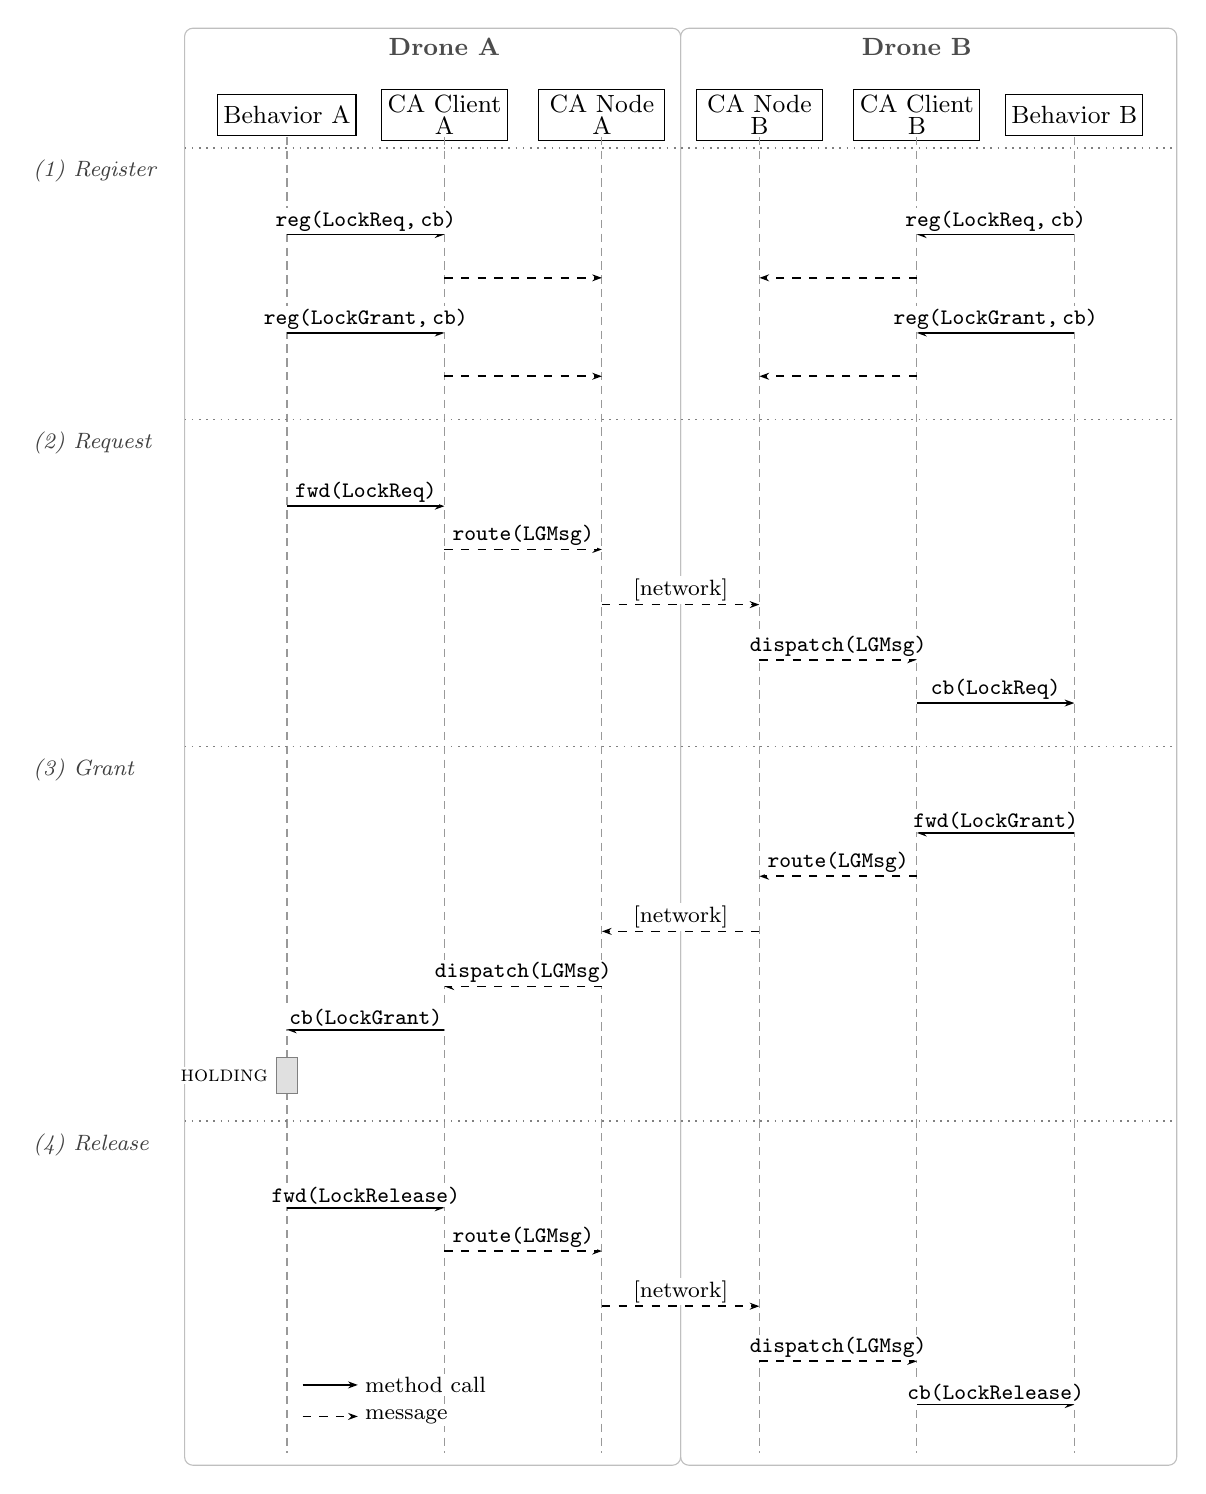
\begin{tikzpicture}[
  yscale=1,
  font=\small,
  box/.style={draw, fill=white, rectangle, minimum width=1.6cm,
              minimum height=0.52cm, align=center, inner sep=2pt},
  ll/.style={densely dashed, black!40},
  arr/.style={-{Stealth[length=3.5pt,width=2.5pt]}, semithick},
  marr/.style={-{Stealth[length=3.5pt,width=2.5pt]}, semithick, dashed},
  narr/.style={-{Stealth[length=3.5pt,width=2.5pt]}, semithick, dashed, black!55},
  lbl/.style={font=\footnotesize, fill=white, inner sep=1pt},
  sep/.style={dotted, black!50, semithick},
  phase/.style={font=\footnotesize\itshape, black!75, fill=white, inner sep=2pt},
]

  \def\xA{0}      % Behavior A (requesting drone)
  \def\xE{2.0}    % CA Client A
  \def\xB{4.0}    % CA Node A
  \def\xC{6.0}    % CA Node B
  \def\xF{8.0}    % CA Client B
  \def\xD{10.0}   % Behavior B (peer drone)

  % --- Participant boxes ---
  \node[box] at (\xA,0) {Behavior A};
  \node[box] at (\xE,0) {\shortstack{CA Client\\[-1pt]A}};
  \node[box] at (\xB,0) {\shortstack{CA Node\\[-1pt]A}};
  \node[box] at (\xC,0) {\shortstack{CA Node\\[-1pt]B}};
  \node[box] at (\xF,0) {\shortstack{CA Client\\[-1pt]B}};
  \node[box] at (\xD,0) {Behavior B};

  % --- Lifelines ---
  \foreach \x in {\xA,\xE,\xB,\xC,\xF,\xD}
    \draw[ll] (\x,-0.28) -- (\x,-17.00);

  % --- Drone grouping outlines ---
  \draw[rounded corners=3pt, black!25]
    (-1.3, 1.1) rectangle (5.0,-17.15);
  \node[font=\small\bfseries, text=black!70, anchor=north]
    at ({(\xA+\xB)/2}, 1.1) {Drone A};

  \draw[rounded corners=3pt, black!25]
    (5.0, 1.1) rectangle (11.3,-17.15);
  \node[font=\small\bfseries, text=black!70, anchor=north]
    at ({(\xC+\xD)/2}, 1.1) {Drone B};

  % ======== (1) Register ========
  \draw[sep] (-1.3,-0.42) -- (11.3,-0.42);
  \node[phase, anchor=north west] at (-3.3,-0.50) {(1) Register};

  % Drone A: method call to CA Client, then message to CA Node
  \draw[arr]  (\xA,-1.52) -- (\xE,-1.52)
    node[lbl, above, midway] {\texttt{reg(LockReq,\,cb)}};
  \draw[marr] (\xE,-2.07) -- (\xB,-2.07);
    % node[lbl, above, midway] {\texttt{reg(LockReq,\,cb)}};
  \draw[arr]  (\xA,-2.77) -- (\xE,-2.77)
    node[lbl, above, midway] {\texttt{reg(LockGrant,\,cb)}};
  \draw[marr] (\xE,-3.32) -- (\xB,-3.32);
    % node[lbl, above, midway] {\texttt{reg(LockGrant,\,cb)}};

  % Drone B: symmetrically
  \draw[arr]  (\xD,-1.52) -- (\xF,-1.52)
    node[lbl, above, midway] {\texttt{reg(LockReq,\,cb)}};
  \draw[marr] (\xF,-2.07) -- (\xC,-2.07);
    % node[lbl, above, midway] {\texttt{reg(LockReq,\,cb)}};
  \draw[arr]  (\xD,-2.77) -- (\xF,-2.77)
    node[lbl, above, midway] {\texttt{reg(LockGrant,\,cb)}};
  \draw[marr] (\xF,-3.32) -- (\xC,-3.32);
    % node[lbl, above, midway] {\texttt{reg(LockGrant,\,cb)}};

  % ======== (2) Request ========
  \draw[sep] (-1.3,-3.87) -- (11.3,-3.87);
  \node[phase, anchor=north west] at (-3.3,-3.95) {(2) Request};

  \draw[arr]  (\xA,-4.97) -- (\xE,-4.97)
    node[lbl, above, midway] {\texttt{fwd(LockReq)}};
  \draw[marr] (\xE,-5.52) -- (\xB,-5.52)
    node[lbl, above, midway] {\texttt{route(LGMsg)}};
  \draw[marr] (\xB,-6.22) -- (\xC,-6.22)
    node[lbl, above, midway, text=black] {[network]};
  \draw[marr] (\xC,-6.92) -- (\xF,-6.92)
    node[lbl, above, midway] {\texttt{dispatch(LGMsg)}};
  \draw[arr]  (\xF,-7.47) -- (\xD,-7.47)
    node[lbl, above, midway] {\texttt{cb(LockReq)}};

  % ======== (3) Grant ========
  \draw[sep] (-1.3,-8.02) -- (11.3,-8.02);
  \node[phase, anchor=north west] at (-3.3,-8.10) {(3) Grant};

  \draw[arr]  (\xD,-9.12) -- (\xF,-9.12)
    node[lbl, above, midway] {\texttt{fwd(LockGrant)}};
  \draw[marr] (\xF,-9.67) -- (\xC,-9.67)
    node[lbl, above, midway] {\texttt{route(LGMsg)}};
  \draw[marr] (\xC,-10.37) -- (\xB,-10.37)
    node[lbl, above, midway, text=black] {[network]};
  \draw[marr] (\xB,-11.07) -- (\xE,-11.07)
    node[lbl, above, midway] {\texttt{dispatch(LGMsg)}};
  \draw[arr]  (\xE,-11.62) -- (\xA,-11.62)
    node[lbl, above, midway] {\texttt{cb(LockGrant)}};

  % HOLDING activation bar on Behavior A
  \fill[black!12] (\xA-0.13,-11.97) rectangle (\xA+0.13,-12.43);
  \draw[black!50] (\xA-0.13,-11.97) rectangle (\xA+0.13,-12.43);
  \node[lbl, left] at (\xA-0.20,-12.20) {\textsc{holding}};

  % ======== (4) Release ========
  \draw[sep] (-1.3,-12.78) -- (11.3,-12.78);
  \node[phase, anchor=north west] at (-3.3,-12.86) {(4) Release};

  \draw[arr]  (\xA,-13.88) -- (\xE,-13.88)
    node[lbl, above, midway] {\texttt{fwd(LockRelease)}};
  \draw[marr] (\xE,-14.43) -- (\xB,-14.43)
    node[lbl, above, midway] {\texttt{route(LGMsg)}};
  \draw[marr] (\xB,-15.13) -- (\xC,-15.13)
    node[lbl, above, midway, text=black] {[network]};
  \draw[marr] (\xC,-15.83) -- (\xF,-15.83)
    node[lbl, above, midway] {\texttt{dispatch(LGMsg)}};
  \draw[arr]  (\xF,-16.38) -- (\xD,-16.38)
    node[lbl, above, midway] {\texttt{cb(LockRelease)}};

  % --- Legend ---
  \draw[arr]  (0.20,-16.13) -- (0.90,-16.13);
  \node[lbl, anchor=west] at (0.95,-16.13) {method call};
  \draw[marr] (0.20,-16.53) -- (0.90,-16.53);
  \node[lbl, anchor=west] at (0.95,-16.53) {message};

\end{tikzpicture}%
}}
\caption{CA Gateway and CA Client message flow in the Collision Avoidance Behavior for a non-conflicting two-drone interaction.
\textit{(1)~Register}: on activation each behavior invokes \texttt{reg()} on its local CA Client (method call); the CA Client forwards the registration to the CA Node (message).
\textit{(2)~Request}: Drone~A calls \texttt{fwd()} on CA Client~A (method), which publishes the request to CA Node~A (message); the request crosses the network to CA Node~B, which dispatches it to CA Client~B (message), invoking Behavior~B's callback (method).
\textit{(3)~Grant}: Behavior~B calls \texttt{fwd()} on CA Client~B (method); the grant travels the reverse path back to Behavior~A; once all grants are received, Behavior~A enters \textsc{holding}.
\textit{(4)~Release}: after completing its path, Drone~A forwards a \code{CAPathLockRelease} via the same chain, unblocking any deferred peers.
Solid arrows denote method calls on the CA Client; dashed arrows denote messages between CA Client and CA Node or between CA Nodes.}
\label{fig:ca_gateway_ca_beh}
\end{figure}

\section{Using the State Interface}

On goal activation, before broadcasting the lock request, the behavior reads the drone's current pose from the State Interface and prepends it to the goal path. This ensures that the lock covers the full corridor from the drone's current position to the first planned waypoint---not just from the first planned waypoint onward---which is the only correct interpretation of ``reserving the path'' at the moment of invocation.

Figure~\ref{fig:ca_state_interface} shows the interaction between the Collision Avoidance Behavior and the State Interface during goal activation. The call occurs before any modelet is sent over the CA Gateway, so the prepended pose is always part of the lock request broadcast to peers.

\begin{figure}[tbh]
\centering
\resizebox{\textwidth}{!}{%
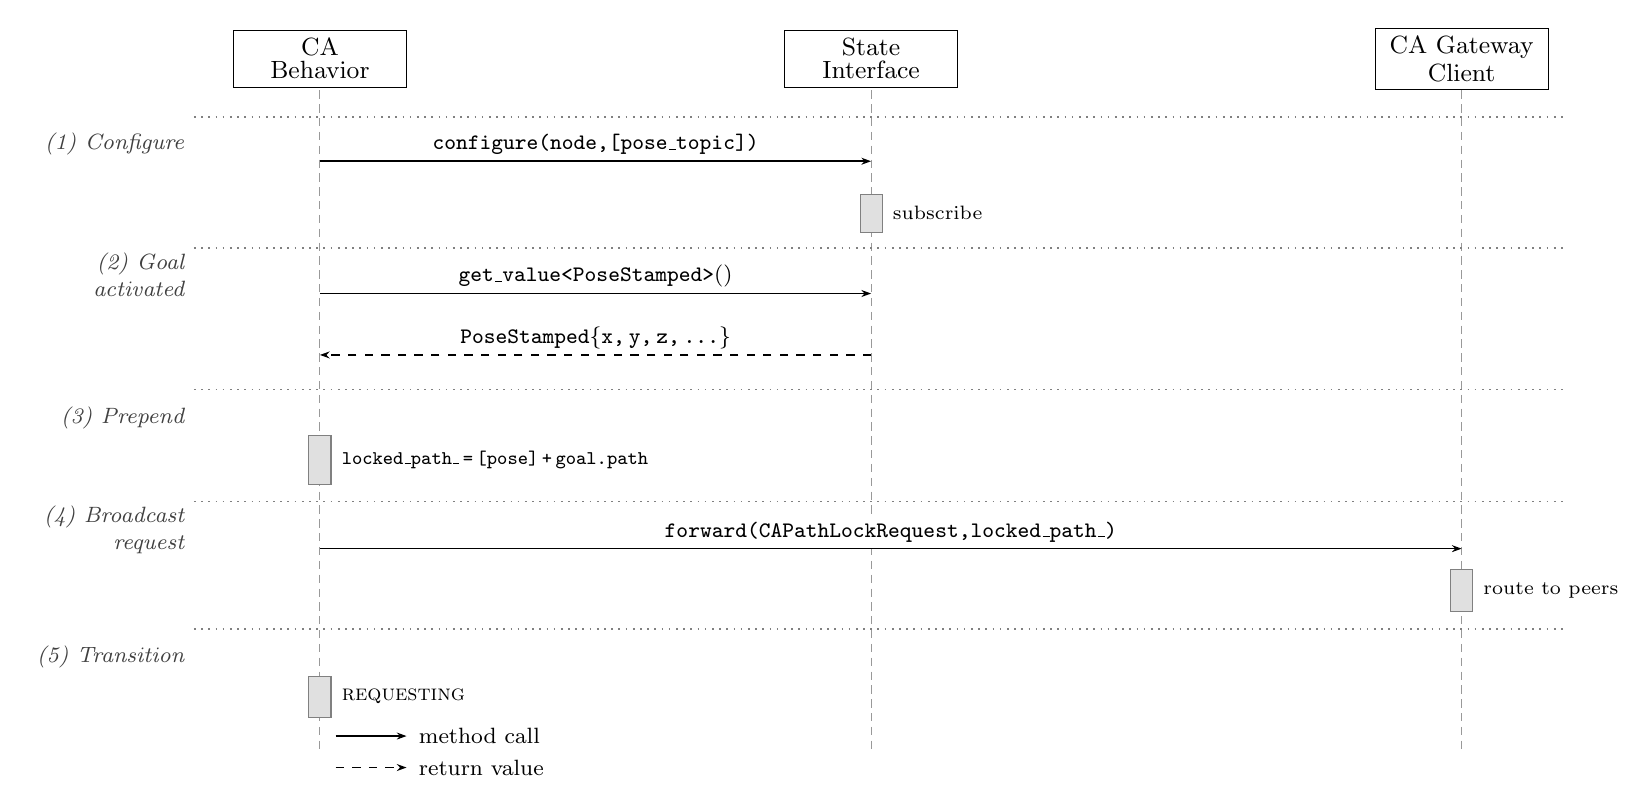
\begin{tikzpicture}[
  font=\small,
  box/.style={draw, fill=white, rectangle, minimum width=2.2cm,
              minimum height=0.56cm, align=center, inner sep=3pt},
  ll/.style={densely dashed, black!40},
  arr/.style={-{Stealth[length=3.5pt,width=2.5pt]}, semithick},
  rarr/.style={-{Stealth[length=3.5pt,width=2.5pt]}, semithick, dashed},
  lbl/.style={font=\footnotesize, fill=white, inner sep=2pt},
  sep/.style={dotted, black!50, semithick},
  phase/.style={font=\footnotesize\itshape, black!75},
]

  \def\xA{0}     % CA Behavior
  \def\xB{7.0}   % State Interface
  \def\xC{14.5}  % CA Gateway Client

  % --- Participant boxes ---
  \node[box] at (\xA,.3) {\shortstack{CA\\[-1pt]Behavior}};
  \node[box] at (\xB,.3) {\shortstack{State\\[-1pt]Interface}};
  \node[box] at (\xC,.3) {\shortstack{CA Gateway\\[-1pt]Client}};

  % --- Lifelines ---
  \foreach \x in {\xA,\xB,\xC}
    \draw[ll] (\x,-0.1) -- (\x,-8.50);

  % ======== (1) Configure ========
  \draw[sep] (-1.6,-0.44) -- (15.8,-0.44);
  \node[phase, anchor=east] at (-1.6,-0.78) {(1) Configure};

  % Arrow A->B: label kept in left half, well clear of B lifeline
  \draw[arr] (\xA,-1.00) -- (\xB,-1.00)
    node[lbl, above, pos=0.5]
      {\shortstack{\texttt{configure(node,}\texttt{[pose\_topic])}}};
  \fill[black!12] (\xB-0.14,-1.42) rectangle (\xB+0.14,-1.90);
  \draw[black!50] (\xB-0.14,-1.42) rectangle (\xB+0.14,-1.90);
  \node[lbl, right] at (\xB+0.20,-1.66) {\scriptsize subscribe};

  % ======== (2) Goal activated ========
  \draw[sep] (-1.6,-2.10) -- (15.8,-2.10);
  \node[phase, anchor=east, align=right] at (-1.6,-2.44) {(2) Goal\\activated};

  % Arrow A->B: label in left half
  \draw[arr] (\xA,-2.68) -- (\xB,-2.68)
    node[lbl, above, pos=0.5]
      {\shortstack{\texttt{get\_value}\texttt{<PoseStamped>}()}};
  % Return arrow B->A: label in right half (near B, away from A lifeline)
  \draw[rarr] (\xB,-3.46) -- (\xA,-3.46)
    node[lbl, above, pos=0.5]
      {\shortstack{\texttt{PoseStamped}\texttt{\{x,\,y,\,z,\,\ldots\}}}};

  % ======== (3) Prepend pose ========
  \draw[sep] (-1.6,-3.90) -- (15.8,-3.90);
  \node[phase, anchor=east] at (-1.6,-4.26) {(3) Prepend};

  \fill[black!12] (\xA-0.14,-4.48) rectangle (\xA+0.14,-5.10);
  \draw[black!50] (\xA-0.14,-4.48) rectangle (\xA+0.14,-5.10);
  \node[lbl, right] at (\xA+0.20,-4.79)
    {\scriptsize\texttt{locked\_path\_\,=\,[pose]\,+\,goal.path}};

  % ======== (4) Broadcast request ========
  \draw[sep] (-1.6,-5.32) -- (15.8,-5.32);
  \node[phase, anchor=east, align=right] at (-1.6,-5.68) {(4) Broadcast\\request};

  % Arrow A->C: label anchored well left of B lifeline (x=7.0) at pos≈0.28 -> x≈4.0
  \draw[arr] (\xA,-5.92) -- (\xC,-5.92)
    node[lbl, above, pos=0.5]
      {\shortstack{\texttt{forward(}\texttt{CAPathLockRequest,}\texttt{locked\_path\_)}}};

  \fill[black!12] (\xC-0.14,-6.18) rectangle (\xC+0.14,-6.72);
  \draw[black!50] (\xC-0.14,-6.18) rectangle (\xC+0.14,-6.72);
  \node[lbl, right] at (\xC+0.20,-6.45) {\scriptsize route to peers};

  % ======== (5) Transition ========
  \draw[sep] (-1.6,-6.94) -- (15.8,-6.94);
  \node[phase, anchor=east] at (-1.6,-7.30) {(5) Transition};

  \fill[black!12] (\xA-0.14,-7.54) rectangle (\xA+0.14,-8.06);
  \draw[black!50] (\xA-0.14,-7.54) rectangle (\xA+0.14,-8.06);
  \node[lbl, right] at (\xA+0.20,-7.80) {\textsc{requesting}};

  % --- Legend ---
  \draw[arr]  (0.20,-8.3) -- (1.10,-8.3);
  \node[lbl, anchor=west] at (1.18,-8.3) {method call};
  \draw[rarr] (0.20,-8.7) -- (1.10,-8.7);
  \node[lbl, anchor=west] at (1.18,-8.7) {return value};

\end{tikzpicture}
}% end resizebox
\caption{Interaction between the Collision Avoidance Behavior and the State Interface during goal activation.
\textit{(1)~Configure}: on node startup the behavior calls \code{configure} on the State Interface, which subscribes to the drone's \code{self\_localization/pose} topic.
\textit{(2)~Goal activated}: when a new \code{CollisionAvoidance} goal arrives, the behavior calls \code{get\_value} to obtain the latest cached \code{PoseStamped}.
\textit{(3)~Prepend}: the returned pose is inserted at the front of the goal path, forming \code{locked\_path\_}---the full corridor from the drone's current position to the last waypoint.
\textit{(4)~Broadcast request}: the extended path is embedded in a \code{CAPathLockRequest} and forwarded to all known peers via the CA Gateway Client.
\textit{(5)~Transition}: the behavior enters the \textsc{requesting} state and waits for grants.}
\label{fig:ca_state_interface}
\end{figure}

\section{Motion orchestration}

The behavior orchestrates the full acquire-execute-release lifecycle by delegating motion to the existing \code{GoToWaypoint} action client:

\begin{enumerate}
  \item \textbf{REQUESTING\_LOCK} --- broadcast \code{CAPathLockRequest} to all known peers; wait until a \code{CAPathLockGrant} has been received from every peer.
  \item \textbf{HOLDING\_LOCK} --- send the \code{GoToWaypoint} goal; transition to EXECUTING\_MOTION.
  \item \textbf{EXECUTING\_MOTION} --- wait for the \code{GoToWaypoint} result.
  \item \textbf{RELEASING\_LOCK} --- broadcast \code{CAPathLockRelease}; flush deferred grants; return success.
\end{enumerate}

On \code{on\_pause()}, the in-flight \code{GoToWaypoint} is cancelled and the lock is released so peers are not blocked while the drone is paused. On \code{on\_resume()}, the lock is re-acquired from scratch before motion restarts.

%%%%%%%%%%%%%%%%%%%%%%%%%%%%%%%%%%%%%%%%%%%%%%%%%%%%%%%%%%%%%%%%%%%%%%%%%%%%%

\chapter{Collective Awareness in the Inspection Scenarios}
\label{ch:scenarios}

This chapter traces each use case family defined in D7.1 and D7.2 to the components that enable it.

\section{Normal operation: the complete inspection loop}

The default scenario (D7.1 Section~7.1) requires the swarm to divide the inspection area, navigate safely to each panel, take images, and return. The implemented components cover steps~5 and~6 of that scenario (task distribution and safe trajectory planning):

\begin{enumerate}
  \item The mission script calls \code{drone.auction(...)} with the inspection targets.
  \item Each drone's \code{AuctionBehavior} reads its current pose from the State Interface, computes costs via the \code{coordinate\_item} plugin, and broadcasts a \code{Bid} modelet through the CA Gateway.
  \item Every drone runs \code{greedy\_sequential} on the received bids; the auction converges and results are asserted in the knowledge base.
  \item The KB monitor detects the \code{is\_assigned\_to} triples and resumes each drone's mission interpreter.
  \item Each drone invokes \code{CollisionAvoidanceBehavior} with its planned path. If paths conflict, the pairwise lock protocol reaches consensus on access order before motion begins.
  \item Drones navigate to their targets; on completion, path locks are released and deferred peers proceed.
\end{enumerate}

This loop satisfies IT-FR-002, IT-FR-027, IT-FR-031, and IT-FR-032 from D7.2.

\section{UC1: Robot failure and swarm replanning}

UC1 (D7.1 Section~7.3) covers battery decay (UC1.1) and GPS loss (UC1.2) scenarios:

\begin{itemize}
  \item \textbf{Failure detection:} The failing drone's battery level is cached by its State Interface and read by the Power Management cognitive function. When an abnormal decay is detected, the fact \code{drone0 battery\_status critical} is asserted in the knowledge base.
  \item \textbf{Mission reaction:} A KB monitor handler triggers an emergency landing sequence and publishes a \code{MissionUpdate} removing the drone from the active fleet.
  \item \textbf{Replanning:} The mission monitor triggers a new auction over the uncovered targets. The \code{AuctionBehavior} reallocates them among the remaining drones, computing fresh costs from each drone's current pose via the State Interface.
\end{itemize}

This satisfies IT-FR-003 (system replanning) and IT-FR-016 (failure resilience).

\section{UC2: Emergency landing with collision avoidance}

UC2 (D7.1 Section~7.4) addresses a drone landing inside the inspection area. D7.1 states explicitly that \emph{``drones must maintain a safe distance at all times, so making an emergency landing inside the inspection area means changing the trajectory of nearby drones''} (UC2.1, step~3).

The collision avoidance behavior handles this directly: the failing drone invokes \\\code{CollisionAvoidanceBehavior} with its emergency landing path and broadcasts a \\\code{CAPathLockRequest}. Peers in HOLDING state grant the request immediately (they release and yield); peers in REQUESTING state grant if the failing drone has lexicographic priority. Once the failing drone broadcasts \code{CAPathLockRelease}, deferred peers resume.

This is the scenario described in D7.3 Section~5.3 (\emph{Social Choice for Emergency Landing}), where the Organisation Handling subsystem coordinates agent behaviour around an emergency using modelets. The \code{pairwise\_path\_lock\_plugin} is the concrete Aerostack2 implementation of that coordination pattern.

%%%%%%%%%%%%%%%%%%%%%%%%%%%%%%%%%%%%%%%%%%%%%%%%%%%%%%%%%%%%%%%%%%%%%%%%%%%%%

\section{End-to-end component interaction}

The components described in Chapters~\ref{ch:ca}--\ref{ch:ca_beh} interact as an integrated collective awareness system. The following traces the complete inspection cycle for a two-drone fleet, cross-referencing each component:

\begin{enumerate}
  \item A mission script calls \code{drone0.auction(...)} with the inspection targets.
  \item \code{drone0}'s \code{AuctionBehavior} sends a \code{StartAuction} modelet to \code{drone1} via the \textbf{CA Gateway}.
  \item Both drones read their current pose from their \textbf{State Interface} and compute costs via the \code{coordinate\_item} plugin.
  \item Both drones broadcast \code{Bid} modelets via the \textbf{CA Gateway} and run \code{greedy\_sequential}. The auction converges; results are asserted in the \textbf{KB} via \code{KBInterface}.
  \item The \textbf{KB monitor} detects the \code{is\_assigned\_to} triples and resumes each drone's mission interpreter.
  \item Each drone calls \code{CollisionAvoidanceBehavior}, which reads the current pose from the \textbf{State Interface} and prepends it to the goal path.
  \item Each drone broadcasts a \code{CAPathLockRequest} via the \textbf{CA Gateway}. If the paths conflict, the drone with the smaller namespace acquires the lock first and begins navigating; the other waits.
  \item On reaching its target, each drone broadcasts \code{CAPathLockRelease} via the \textbf{CA Gateway}, allowing the deferred peer to proceed.
\end{enumerate}

\section{Configuration}

Each component is configured via standard ROS~2 YAML parameter files. The key parameters are:

\begin{table}[h!]
\centering
\renewcommand{\arraystretch}{1.2}
\caption{Key configuration parameters}
\label{tab:params}
\begin{tabular}{|l|l|l|}\hline
\tabtitle{Component} & \tabtitle{Parameter} & \tabtitle{Default} \\ \hline \hline
\bko CA Gateway & \code{out\_messages\_topic} & \code{gateway\_out} \\ \hline
\bko CA Gateway & \code{register\_module\_service\_name} & \code{register\_module} \\ \hline
\bko Auction & \code{plugin\_name} & \code{greedy\_sequential} \\ \hline
\bko Auction & \code{state\_component} & \code{[]} \\ \hline
\bko Collision Avoidance & \code{plugin\_name} & \code{pairwise\_path\_lock} \\ \hline
\bko Collision Avoidance & \code{safety\_distance} & \code{1.5}~m \\ \hline
\end{tabular}
\renewcommand{\arraystretch}{1}
\end{table}

%%%%%%%%%%%%%%%%%%%%%%%%%%%%%%%%%%%%%%%%%%%%%%%%%%%%%%%%%%%%%%%%%%%%%%%%%%%%%

\chapter{Conclusions}

This deliverable has reported the implementation of the CORESENSE Drone Inspection Testbed (TB2) in Aerostack2, following the infrastructure-first narrative of the D7.3 Collective Awareness Architecture.

The CA Gateway and CA Client (\code{as2\_ca}) implement the D7.3 Communication Interface subsystem: per-agent namespaced topics, automatic peer discovery, and type-dispatched modelet routing provide the intelligible communication channel that collective models require. On top of this, the Knowledge Base Interface (\code{as2\_core}, \code{as2\_python\_api}) provides the persistent, semantic integration layer: behaviors assert facts about mission events and collective decisions, and KB monitor handlers react to those facts to drive mission-level replanning.

The Auction Behavior and the Collision Avoidance Behavior then show how Aerostack2 behaviors function as CORESENSE cognitive modules: each maintains models (cost estimates, planned paths, or peer-observed paths), applies an engine (the greedy-sequential algorithm, the pairwise path-lock protocol), and exchanges modelets through the CA Gateway. The Auction Behavior uses the gateway for bid exchange, the State Interface for self-model data (current pose for cost computation), and the KB Interface to ground the assignment in the knowledge base. The Collision Avoidance Behavior uses the gateway for lock-request exchange and the State Interface to prepend the current position to the path before locking.

Together, these components realise the four use-case families of D7.1: swarm replanning after robot failure (UC1) via re-auction triggered by KB events, safe emergency landing (UC2) via the consensus-based path-lock protocol, discrepancy detection through collective sensing (UC3) via CA Gateway exchange and KB integration, and image quality assurance (UC4) via KB-triggered partial re-auction. They satisfy the D7.2 requirements for collaborative planning, system replanning, failure resilience, information sharing, swarm size awareness, trajectory collective-awareness, and security distance.

The modular plugin architecture ensures that alternative auction strategies, cost functions, and path-lock protocols can be substituted without modifying the behavior infrastructure, allowing the testbed to evolve as the CORESENSE cognitive module library grows.

%%%%%%%%%%%%%%%%%%%%%%%%%%%%%%%%%%%%%%%%%%%%%%%%%%%%%%%%%%%%%%%%%%%%%%%%%%%%%

\bibliography{library}
\bibliographystyle{apalike}

\finalcover

\end{document}
